\section{\textbf{APPENDIX SNAHYP CURVE}} \label{APPENDIX SNAHYP CURVE}


\subsection       {Plot of SnaHyp curve
	[\ref  {01-img-Plot of SnaHyp curve.pdf} ] }
\label{ssec-01-img-Plot of SnaHyp curve.pdf}

\subsection       {SnaHyp Radius of Curvature
	[\ref      {02-img-SnaHyp Radius of Curvature.pdf}] }
\label{ssec-02-img-SnaHyp Radius of Curvature.pdf}

\subsection       {SnaHyp Validation in LinuxCNC
	[\ref      {03-img-SnaHyp-Validation-in-LinuxCNC.png} ] }
\label{ssec-03-img-SnaHyp-Validation-in-LinuxCNC.png}

\subsection     {SnaHyp Direction of Travel 3D
	[\ref      {04-img-SnaHyp Direction of Travel 3D.pdf} ] }
\label{ssec-04-img-SnaHyp Direction of Travel 3D.pdf}

\subsection       {SnaHyp First and Second Order Taylors App
	[\ref      {05-img-SnaHyp-First-and-Second-Order-Taylors-Approx.pdf}] }
\label{ssec-05-img-SnaHyp-First-and-Second-Order-Taylors-Approx.pdf}

\subsection       {SnaHyp First minus Second Order Taylors App
	[\ref      {06-img-SnaHyp-First-minus-Second-Order-Taylors-Approx.pdf}] }
\label{ssec-06-img-SnaHyp-First-minus-Second-Order-Taylors-Approx.pdf}

\subsection       {SnaHyp Separate First Second Order Taylors App
	[\ref      {07-img-SnaHyp-Separation-First-and-Second-Order-Taylors-Approx.pdf} ] }
\label{ssec-07-img-SnaHyp-Separation-First-and-Second-Order-Taylors-Approx.pdf}

\subsection       {SnaHyp Separation SAL and SCL
	[\ref      {08-img-SnaHyp-Separation-SAL-and-SCL.pdf}] }
\label{ssec-08-img-SnaHyp-Separation-SAL-and-SCL.pdf}

\subsection       {SnaHyp Chord-error in close view 2 scales
	[\ref      {09-img-SnaHyp-Chord-error-in-close-view-2-scales.pdf}] }
\label{ssec-09-img-SnaHyp-Chord-error-in-close-view-2-scales.pdf}

\subsection       {SnaHyp Four Components Feedrate Limit
	[\ref      {10-img-SnaHyp-Four-Components-Feedrate-Limit.pdf} ] }
\label{ssec-10-img-SnaHyp-Four-Components-Feedrate-Limit.pdf}

\subsection    {SnaHyp FrateCommand FrateLimit and Curr-Frate
	[\ref      {11-img-SnaHyp-FrateCommand-FrateLimit-and-Curr-Frate.pdf}] }
\label{ssec-11-img-SnaHyp-FrateCommand-FrateLimit-and-Curr-Frate.pdf}

\subsection     {SnaHyp FeedRateLimit minus CurrFeedRate
	[\ref      {12-img-SnaHyp-FeedRateLimit-minus-CurrFeedRate.pdf} ] }
\label{ssec-12-img-SnaHyp-FeedRateLimit-minus-CurrFeedRate.pdf}

\subsection     {SnaHyp FC20-Nominal X and Y Feedrate Profiles
	[\ref      {13-img-SnaHyp-FC20-Nominal-X-and-Y-Feedrate-Profiles.pdf} ] }
\label{ssec-13-img-SnaHyp-FC20-Nominal-X-and-Y-Feedrate-Profiles.pdf}

\subsection     {SnaHyp FC20 Nominal Tangential Acceleration
	[\ref      {14-img-SnaHyp-FC20-Nominal-Tangential-Acceleration.pdf} ] }
\label{ssec-14-img-SnaHyp-FC20-Nominal-Tangential-Acceleration.pdf}

\subsection     {SnaHyp FC20 Nominal Rising S-Curve Profile
	[\ref      {15-img-SnaHyp-FC20-Nominal-Rising-S-Curve-Profile.pdf} ] }
\label{ssec-15-img-SnaHyp-FC20-Nominal-Rising-S-Curve-Profile.pdf}

\subsection     {SnaHyp FC20 Nominal Falling S-Curve Profile
	[\ref      {16-img-SnaHyp-FC20-Nominal-Falling-S-Curve-Profile.pdf}] }
\label{ssec-16-img-SnaHyp-FC20-Nominal-Falling-S-Curve-Profile.pdf}

\subsection       {SnaHyp FC10 Colored Feedrate Profile ngcode
	[\ref      {17-img-SnaHyp-FC10-Colored-Feedrate-Profile-data_ngcode.png} ] }
\label{ssec-17-img-SnaHyp-FC10-Colored-Feedrate-Profile-data_ngcode.png}

\subsection       {SnaHyp FC20 Colored Feedrate Profile ngcode
	[\ref      {18-img-SnaHyp-FC20-Colored-Feedrate-Profile-data_ngcode.png} ] }
\label{ssec-18-img-SnaHyp-FC20-Colored-Feedrate-Profile-data_ngcode.png}

Continue ...\\

\subsection       {SnaHyp FC25 Colored Feedrate Profile ngcode
	[\ref      {19-img-SnaHyp-FC25-Colored-Feedrate-Profile-data_ngcode.png} ] }
\label{ssec-19-img-SnaHyp-FC25-Colored-Feedrate-Profile-data_ngcode.png}

\subsection       {SnaHyp FC28 Colored Feedrate Profile ngcode
	[\ref      {20-img-SnaHyp-FC28-Colored-Feedrate-Profile-data_ngcode.png} ] }
\label{ssec-20-img-SnaHyp-FC28-Colored-Feedrate-Profile-data_ngcode.png}

\subsection       {SnaHyp FC10 Tangential Acceleration
	[\ref      {21-img-SnaHyp-FC10-Tangential-Acceleration.pdf}] }
\label{ssec-21-img-SnaHyp-FC10-Tangential-Acceleration.pdf}

\subsection       {SnaHyp FC20 Tangential Acceleration
	[\ref      {22-img-SnaHyp-FC20-Tangential-Acceleration.pdf}] }
\label{ssec-22-img-SnaHyp-FC20-Tangential-Acceleration.pdf}

\subsection       {SnaHyp FC30 Tangential Acceleration
	[\ref      {23-img-SnaHyp-FC30-Tangential-Acceleration.pdf}] }
\label{ssec-23-img-SnaHyp-FC30-Tangential-Acceleration.pdf}

\subsection       {SnaHyp FC40 Tangential Acceleration
	[\ref      {24-img-SnaHyp-FC40-Tangential-Acceleration.pdf}] }
\label{ssec-24-img-SnaHyp-FC40-Tangential-Acceleration.pdf}

\subsection       {SnaHyp FC20 Nominal Separation NAL and NCL
	[\ref      {25-img-SnaHyp-FC20-Nominal-Separation-NAL-and-NCL.pdf}] }
\label{ssec-25-img-SnaHyp-FC20-Nominal-Separation-NAL-and-NCL.pdf}

\subsection       {SnaHyp SAL minus SCL for FC10 FC20 FC30 FC40
	[\ref      {26-img-SnaHyp-Difference-SAL-minus-SCL-for-FC10-FC20-FC30-FC40.pdf}] }
\label{ssec-26-img-SnaHyp-Difference-SAL-minus-SCL-for-FC10-FC20-FC30-FC40.pdf}


\subsection       {SnaHyp FC10 FrateCmd CurrFrate X-Frate Y-Frate
	[\ref      {27-img-SnaHyp-FC10-FrateCmd-CurrFrate-X-Frate-Y-Frate.pdf}] }
\label{ssec-27-img-SnaHyp-FC10-FrateCmd-CurrFrate-X-Frate-Y-Frate.pdf}

\subsection       {SnaHyp FC20 FrateCmd CurrFrate X-Frate Y-Frate
	[\ref      {28-img-SnaHyp-FC20-FrateCmd-CurrFrate-X-Frate-Y-Frate.pdf}] }
\label{ssec-28-img-SnaHyp-FC20-FrateCmd-CurrFrate-X-Frate-Y-Frate.pdf}

\subsection       {SnaHyp FC25 FrateCmd CurrFrate X-Frate Y-Frate
	[\ref      {29-img-SnaHyp-FC25-FrateCmd-CurrFrate-X-Frate-Y-Frate.pdf}] }
\label{ssec-29-img-SnaHyp-FC25-FrateCmd-CurrFrate-X-Frate-Y-Frate.pdf}

\subsection       {SnaHyp FC28 FrateCmd CurrFrate X-Frate Y-Frate
	[\ref      {30-img-SnaHyp-FC28-FrateCmd-CurrFrate-X-Frate-Y-Frate.pdf}] }
\label{ssec-30-img-SnaHyp-FC28-FrateCmd-CurrFrate-X-Frate-Y-Frate.pdf}

\subsection       {SnaHyp FC10 Four Components FeedrateLimit
	[\ref      {31-img-SnaHyp-FC10-Four-Components-FeedrateLimit.pdf}] }
\label{ssec-31-img-SnaHyp-FC10-Four-Components-FeedrateLimit.pdf}

\subsection       {SnaHyp FC20 Four Components FeedrateLimit
	[\ref      {32-img-SnaHyp-FC20-Four-Components-FeedrateLimit.pdf}] }
\label{ssec-32-img-SnaHyp-FC20-Four-Components-FeedrateLimit.pdf}

\subsection       {SnaHyp FC25 Four Components FeedrateLimit
	[\ref      {33-img-SnaHyp-FC25-Four-Components-FeedrateLimit.pdf}] }
\label{ssec-33-img-SnaHyp-FC25-Four-Components-FeedrateLimit.pdf}

\subsection       {SnaHyp FC28 Four Components FeedrateLimit
	[\ref      {34-img-SnaHyp-FC28-Four-Components-FeedrateLimit.pdf}]}
\label{ssec-34-img-SnaHyp-FC28-Four-Components-FeedrateLimit.pdf}

\subsection       {SnaHyp Histogram Points FC10 FC20 FC30 FC40
	[\ref      {35-img-SnaHyp-Histogram-Points-FC10-FC20-FC30-FC40.pdf}] }
\label{ssec-35-img-SnaHyp-Histogram-Points-FC10-FC20-FC30-FC40.pdf}

\subsection    {SnaHyp Table distribution of interpolated points
	[\ref      {tab-SnaHyp Table distribution of interpolated points}] }
\label{ssec-tab-SnaHyp Table distribution of interpolated points}

\subsection         {SnaHyp Table FC10-20-30-40 Run Performance data
	[\ref      {tab-app4-SnaHyp-Table-FC10-20-30-40-Run-Performance-data}] }
\label{ssec-tab-app4-SnaHyp-Table-FC10-20-30-40-Run-Performance-data}


%% =====================================================
%% =====================================================
\clearpage
\pagebreak

\begin{figure}
	\caption     {Plot of SnaHyp curve}
	\label{01-img-Plot of SnaHyp curve.pdf}
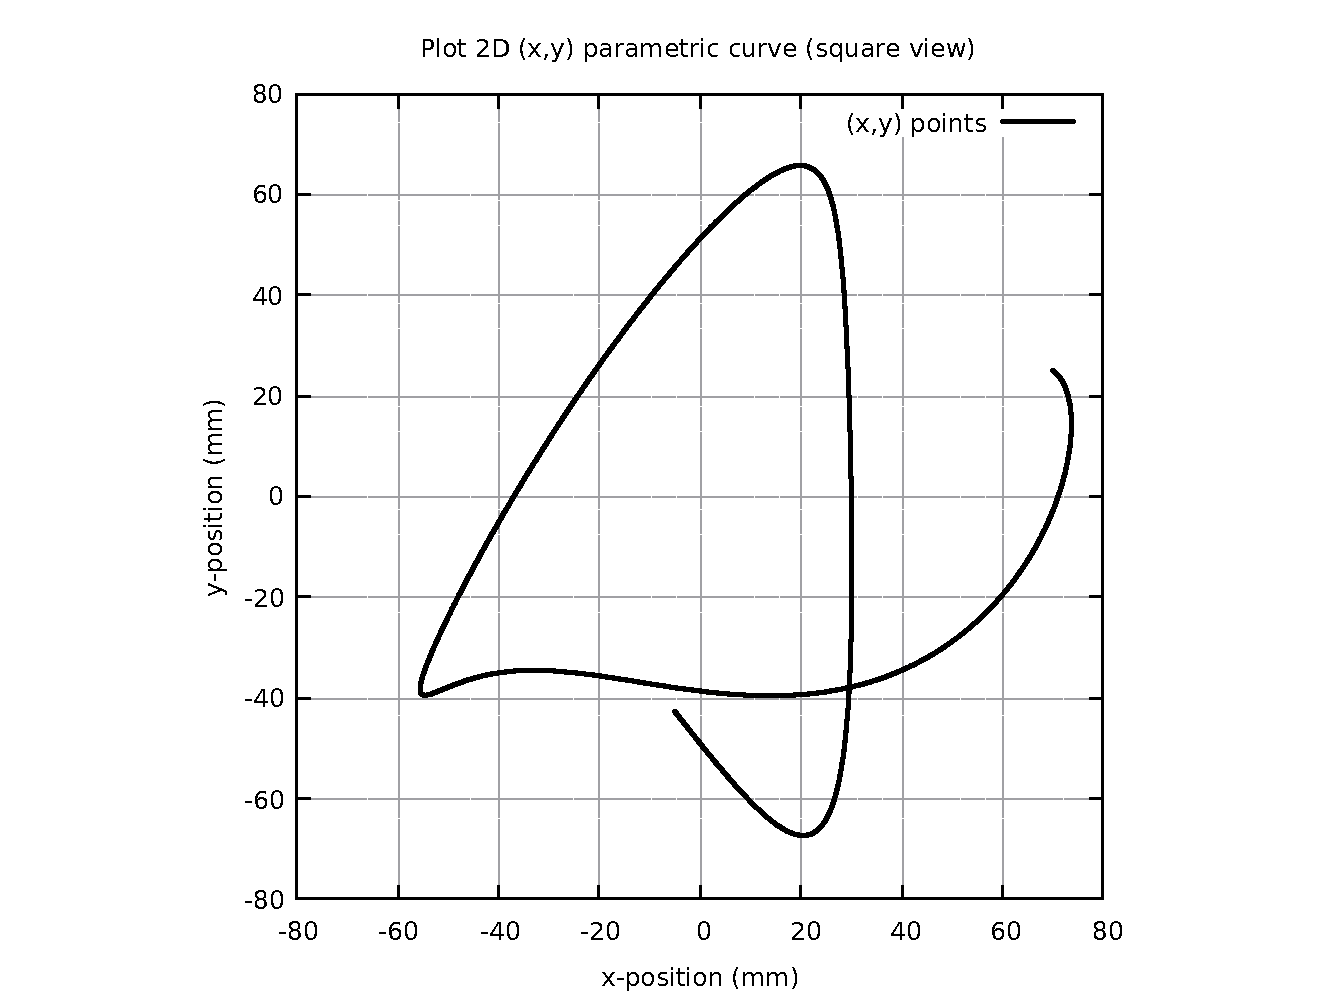
\includegraphics[width=1.00\textwidth]{Chap4/appendix/app-SnaHyp/plots/01-img-Plot of SnaHyp curve.pdf}
\end{figure}	


\begin{figure}
	\caption     {SnaHyp Radius of Curvature}
	\label{02-img-SnaHyp Radius of Curvature.pdf}
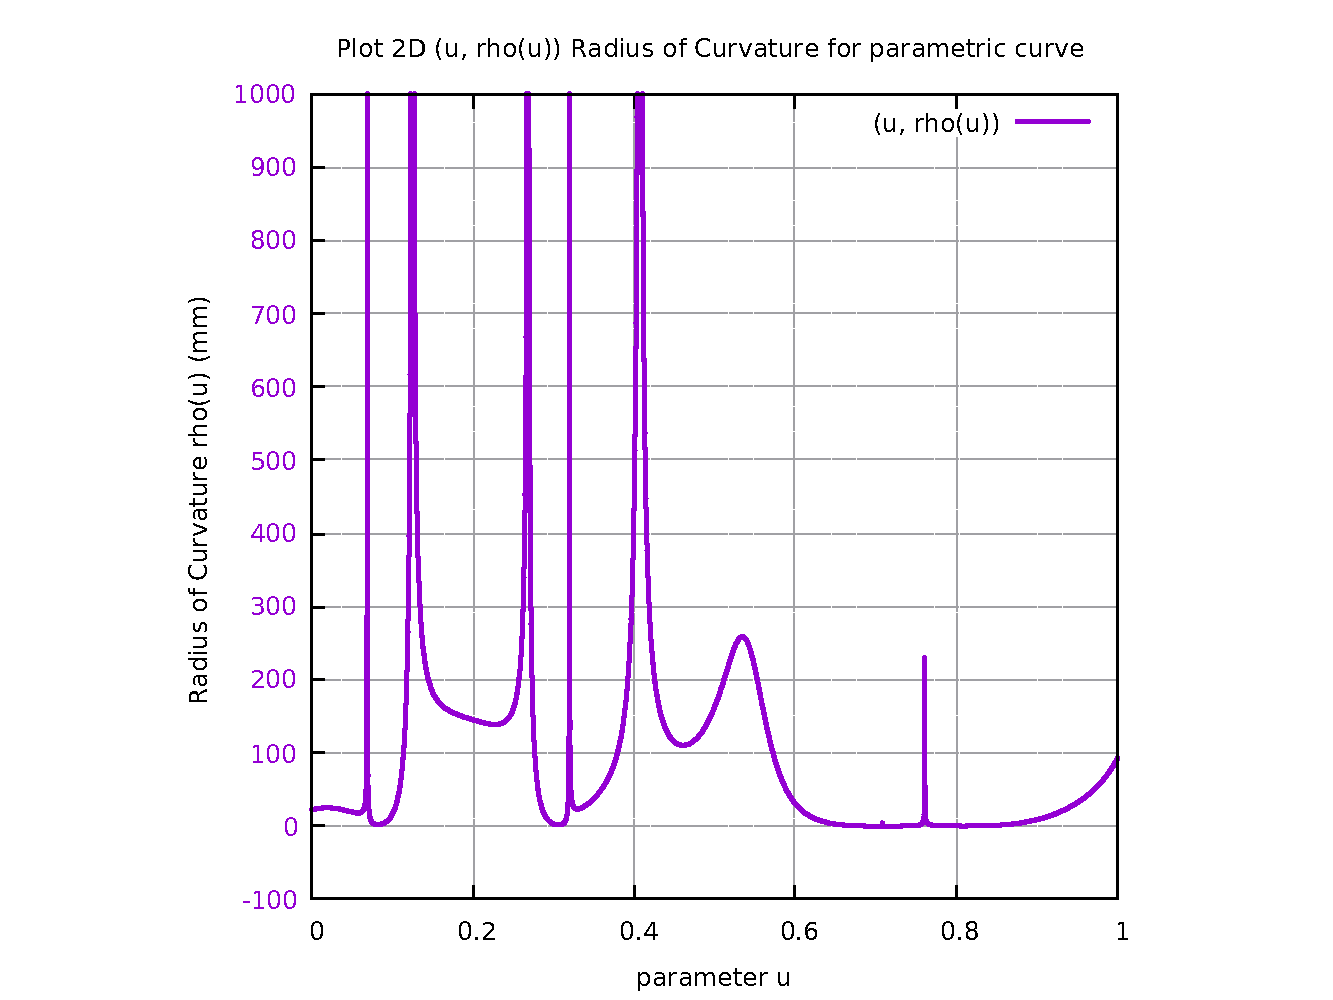
\includegraphics[width=1.00\textwidth]{Chap4/appendix/app-SnaHyp/plots/02-img-SnaHyp Radius of Curvature.pdf} 
\end{figure}	


%% ==================================================
\clearpage
\pagebreak

\begin{figure}
	\caption     {SnaHyp Validation in LinuxCNC}
	\label{03-img-SnaHyp-Validation-in-LinuxCNC.png}
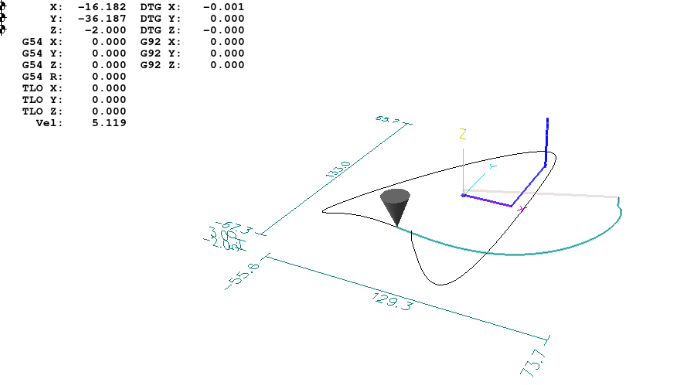
\includegraphics[width=1.00\textwidth]{Chap4/appendix/app-SnaHyp/plots/03-img-SnaHyp-Validation-in-LinuxCNC.png}
\end{figure}


\begin{figure}
	\caption     {SnaHyp Direction of Travel 3D}
	\label{04-img-SnaHyp Direction of Travel 3D.pdf}
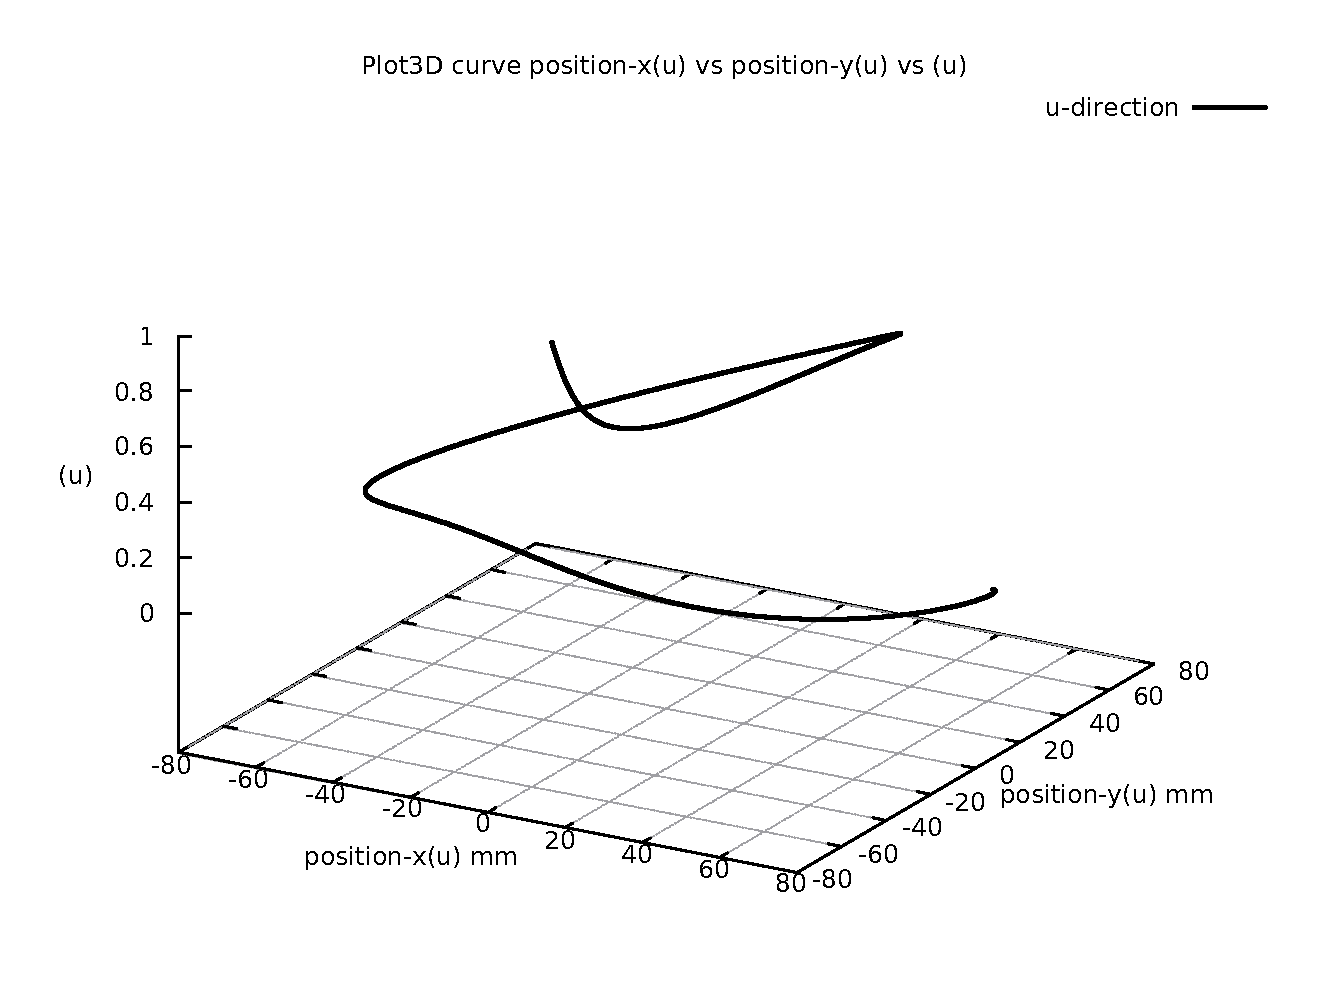
\includegraphics[width=1.00\textwidth]{Chap4/appendix/app-SnaHyp/plots/04-img-SnaHyp Direction of Travel 3D.pdf}
\end{figure}

%% ==================================================
\clearpage
\pagebreak

\begin{figure}
	\caption     {SnaHyp First and Second Order Taylor's Approximation}
	\label{05-img-SnaHyp-First-and-Second-Order-Taylors-Approx.pdf}
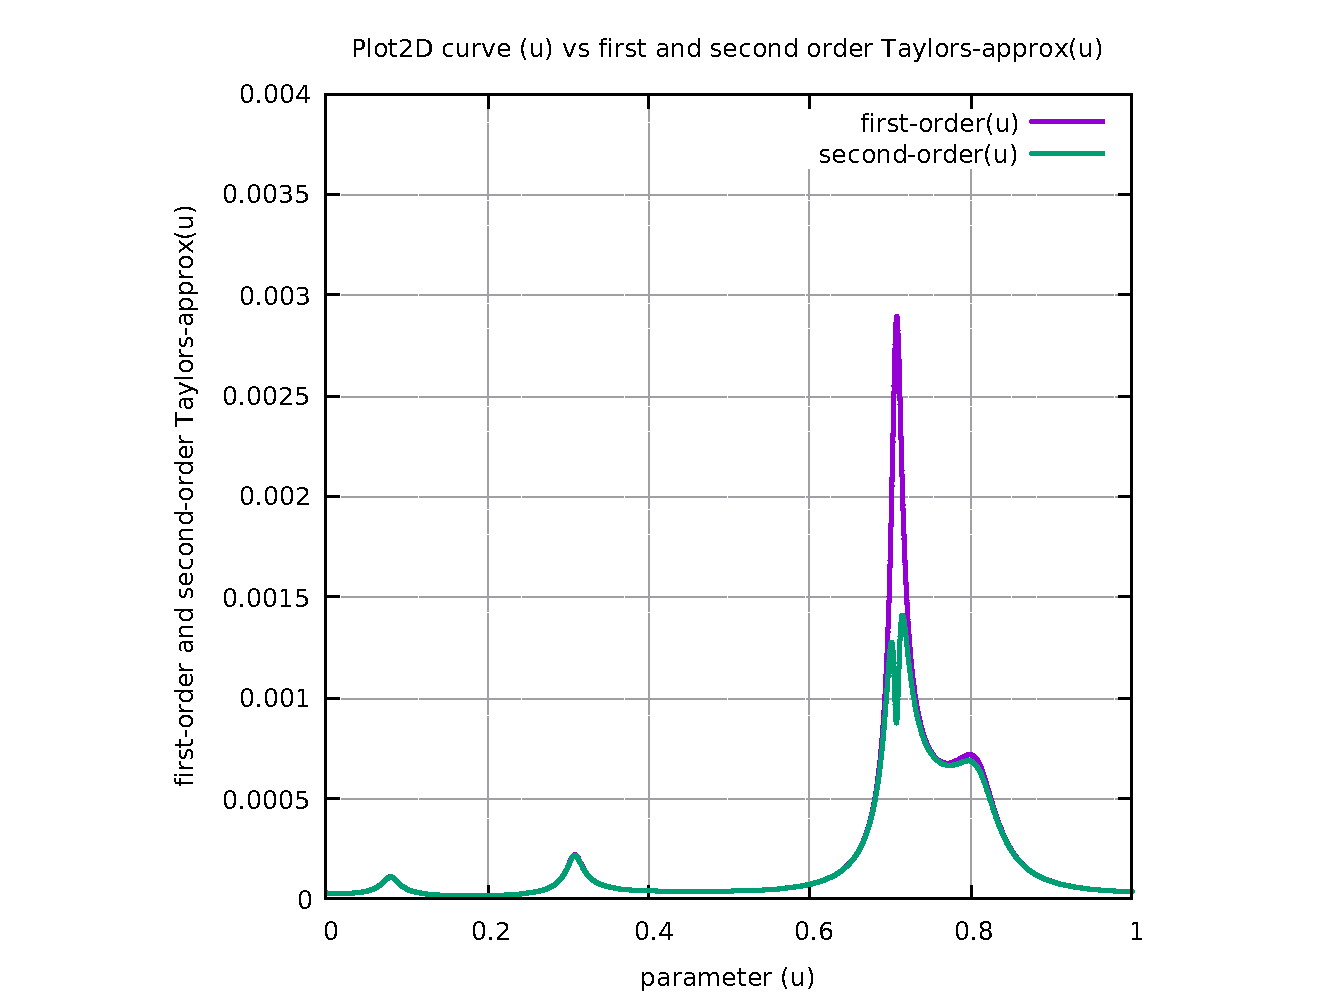
\includegraphics[width=1.00\textwidth]{Chap4/appendix/app-SnaHyp/plots/05-img-SnaHyp-First-and-Second-Order-Taylors-Approx.pdf}
\end{figure}


\begin{figure}
	\caption     {SnaHyp First minus Second Order Taylor's Approximation}
	\label{06-img-SnaHyp-First-minus-Second-Order-Taylors-Approx.pdf}
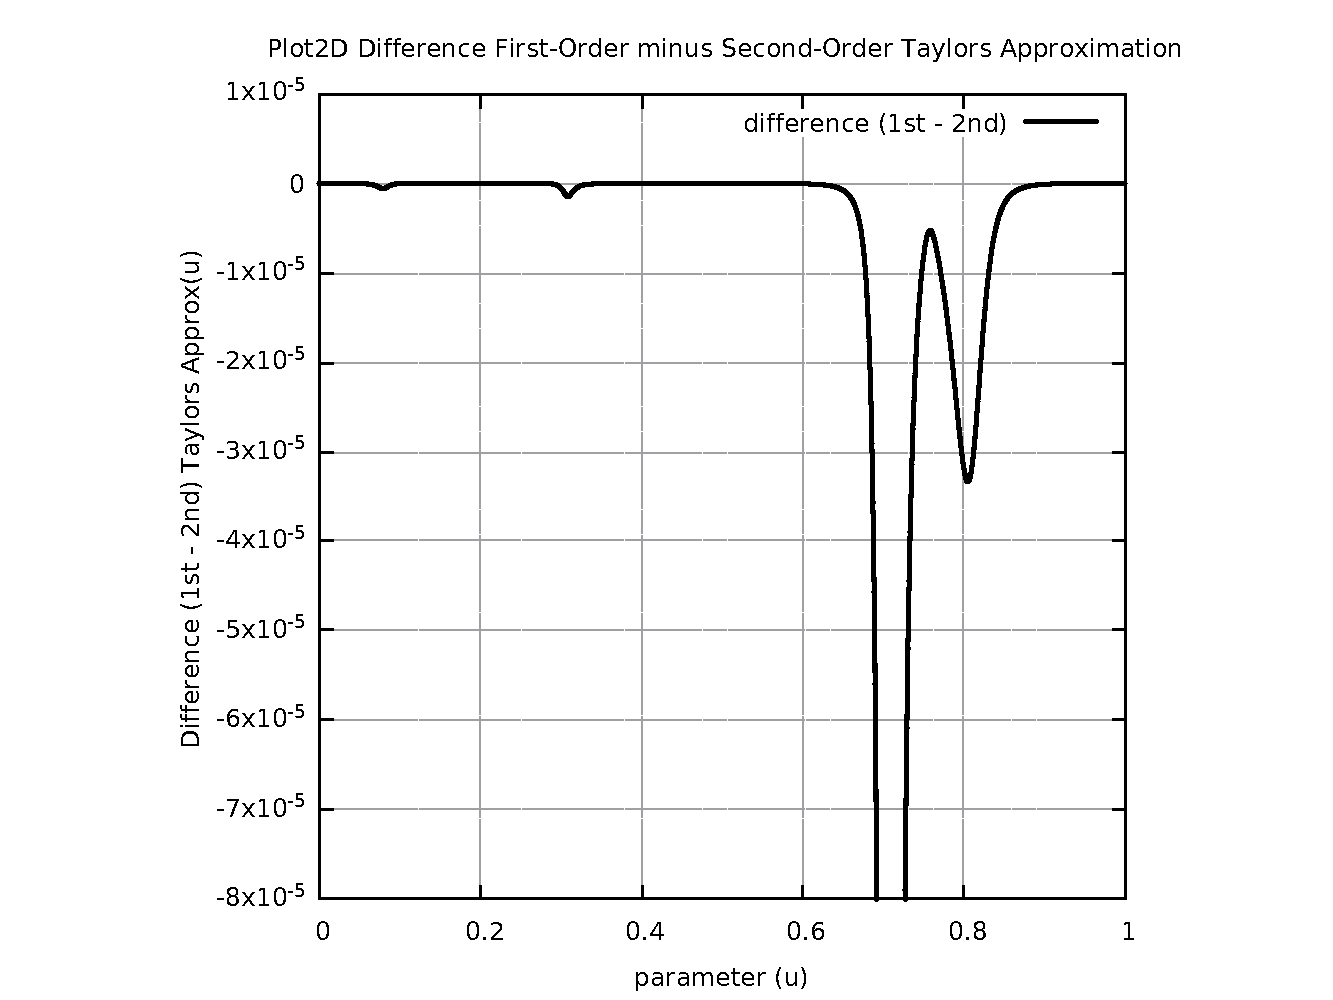
\includegraphics[width=1.00\textwidth]{Chap4/appendix/app-SnaHyp/plots/06-img-SnaHyp-First-minus-Second-Order-Taylors-Approx.pdf}
\end{figure}

%% ==================================================
\clearpage
\pagebreak

\begin{figure}
	\caption     {SnaHyp Separation First and Second Order Taylor's Approximation}
	\label{07-img-SnaHyp-Separation-First-and-Second-Order-Taylors-Approx.pdf}
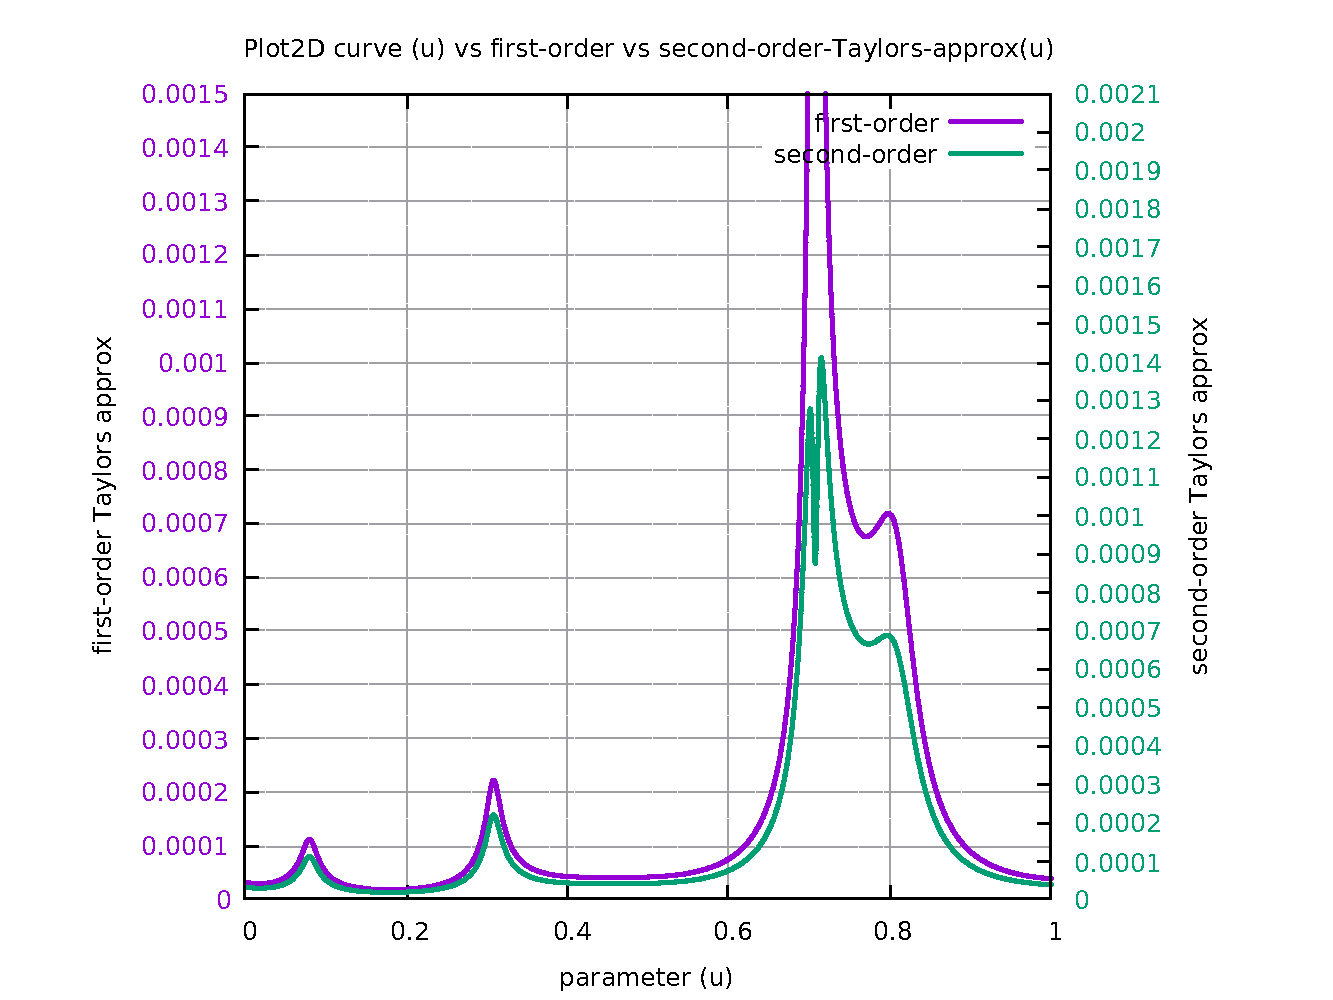
\includegraphics[width=1.00\textwidth]{Chap4/appendix/app-SnaHyp/plots/07-img-SnaHyp-First-and-Second-Order-Taylors-Approx.pdf}
\end{figure}


\begin{figure}
	\caption     {SnaHyp Separation SAL and SCL}
	\label{08-img-SnaHyp-Separation-SAL-and-SCL.pdf}
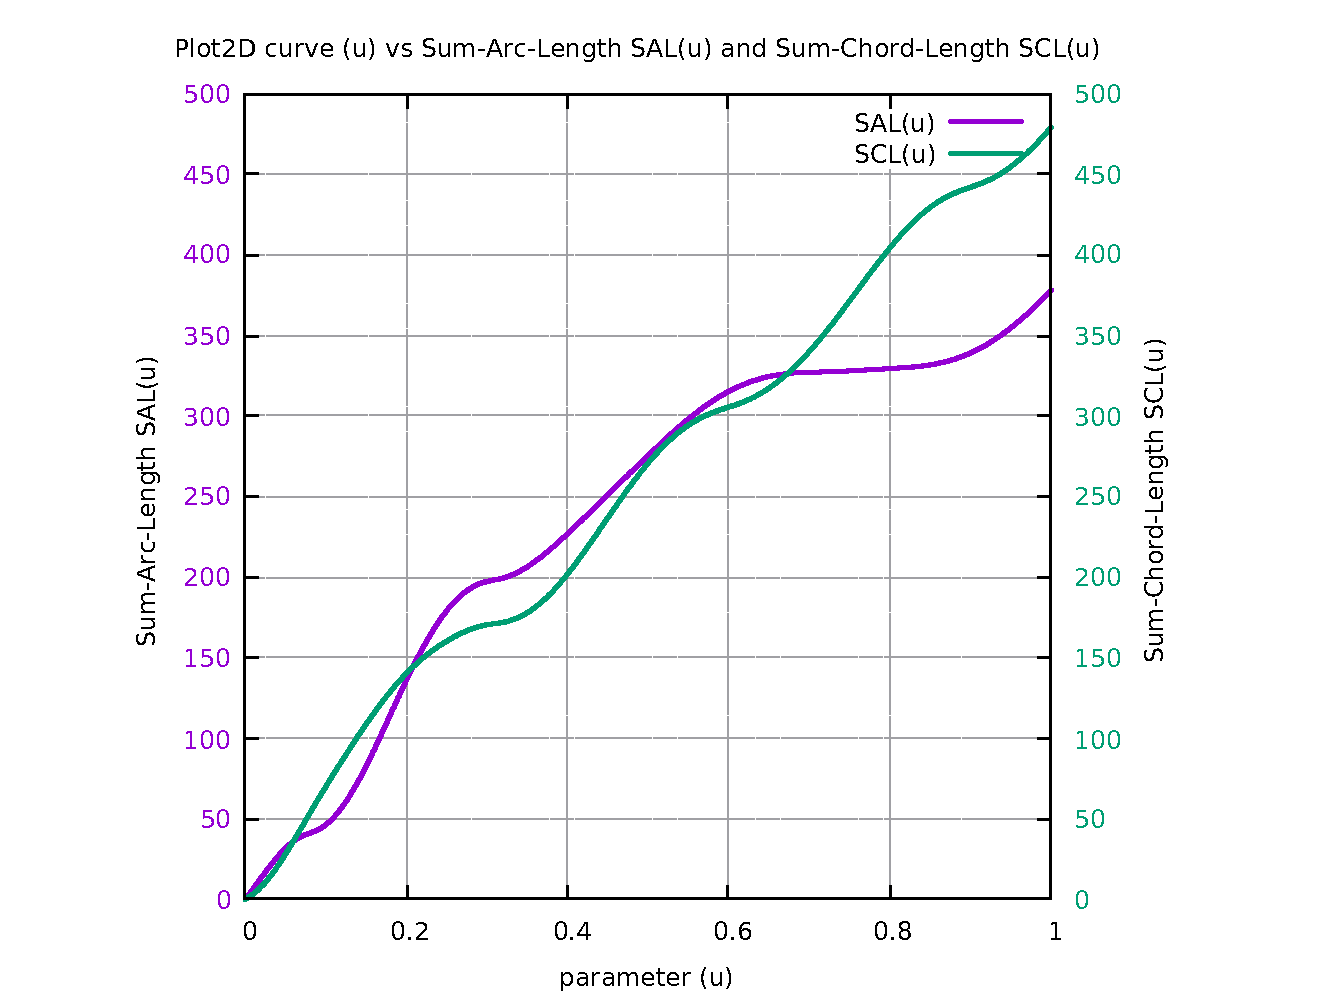
\includegraphics[width=1.00\textwidth]{Chap4/appendix/app-SnaHyp/plots/08-img-SnaHyp-Separation-SAL-and-SCL.pdf}
\end{figure}

%% ==================================================
\clearpage
\pagebreak

\begin{figure}
	\caption     {SnaHyp Chord-error in close view 2 scales}
	\label{09-img-SnaHyp-Chord-error-in-close-view-2-scales.pdf}
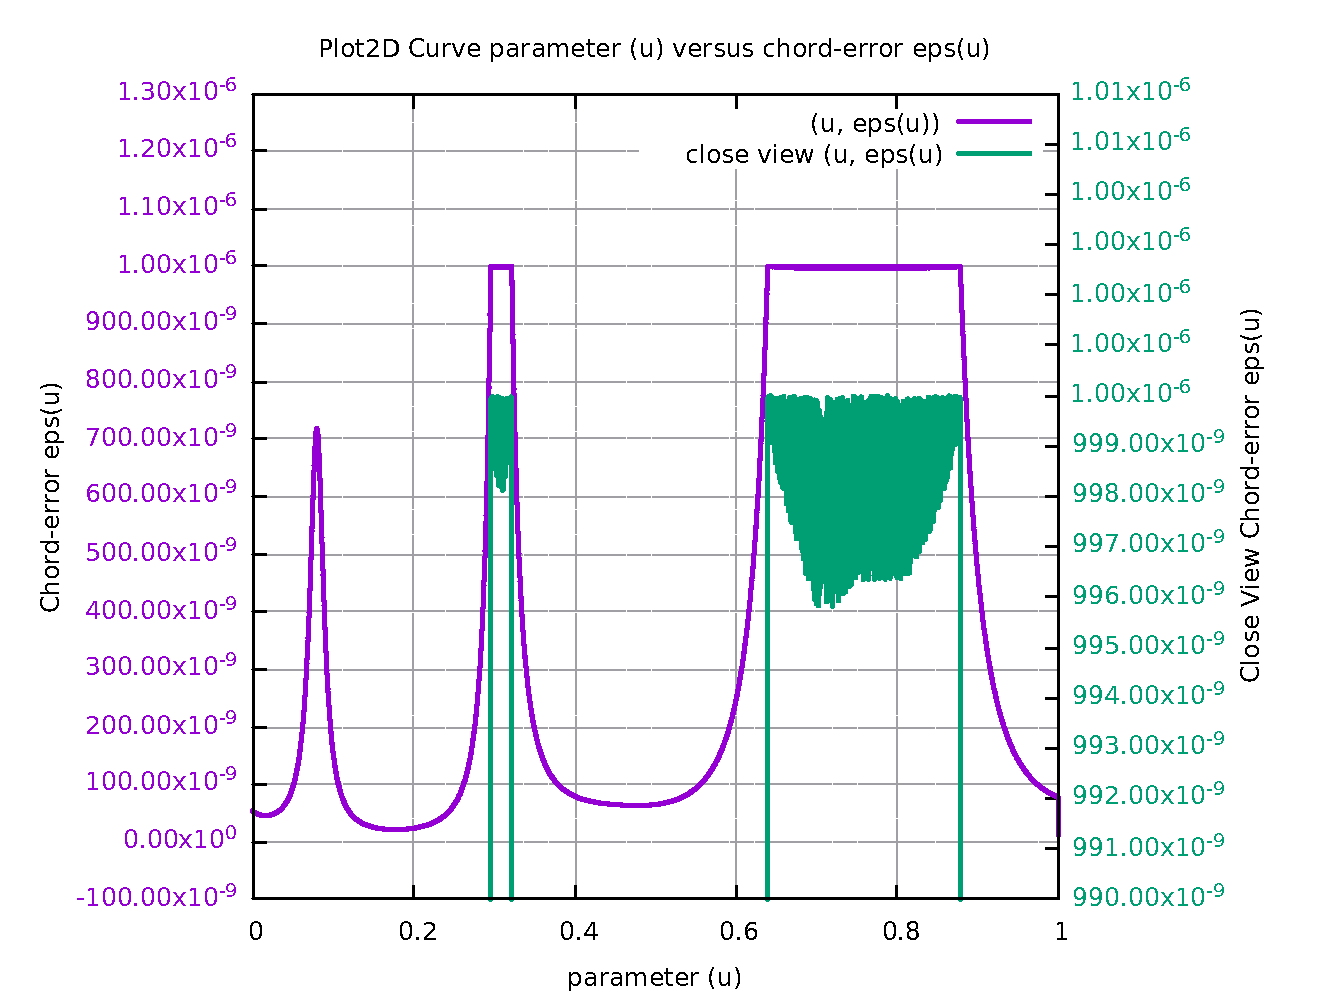
\includegraphics[width=1.00\textwidth]{Chap4/appendix/app-SnaHyp/plots/09-img-SnaHyp-Chord-error-in-close-view-2-scales.pdf}
\end{figure}

\begin{figure}
	\caption     {SnaHyp Four Components Feedrate Limit}
	\label{10-img-SnaHyp-Four-Components-Feedrate-Limit.pdf}
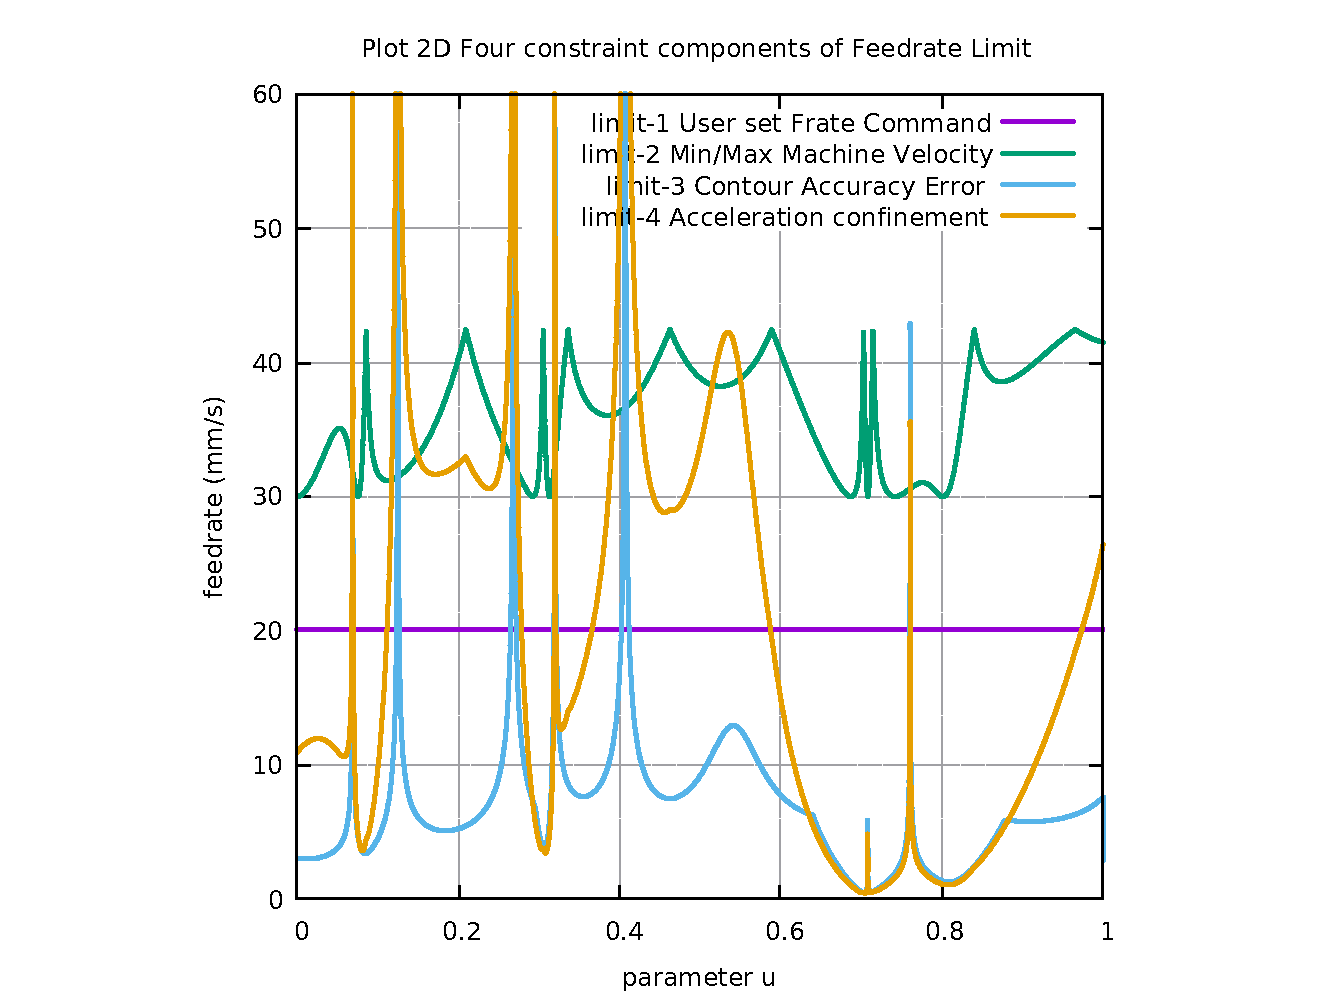
\includegraphics[width=1.00\textwidth]{Chap4/appendix/app-SnaHyp/plots/10-img-SnaHyp-Four-Components-Feedrate-Limit.pdf}
\end{figure}

%% ==================================================
\clearpage
\pagebreak

\begin{figure}
	\caption     {SnaHyp FrateCommand FrateLimit and Curr-Frate}
	\label{11-img-SnaHyp-FrateCommand-FrateLimit-and-Curr-Frate.pdf}
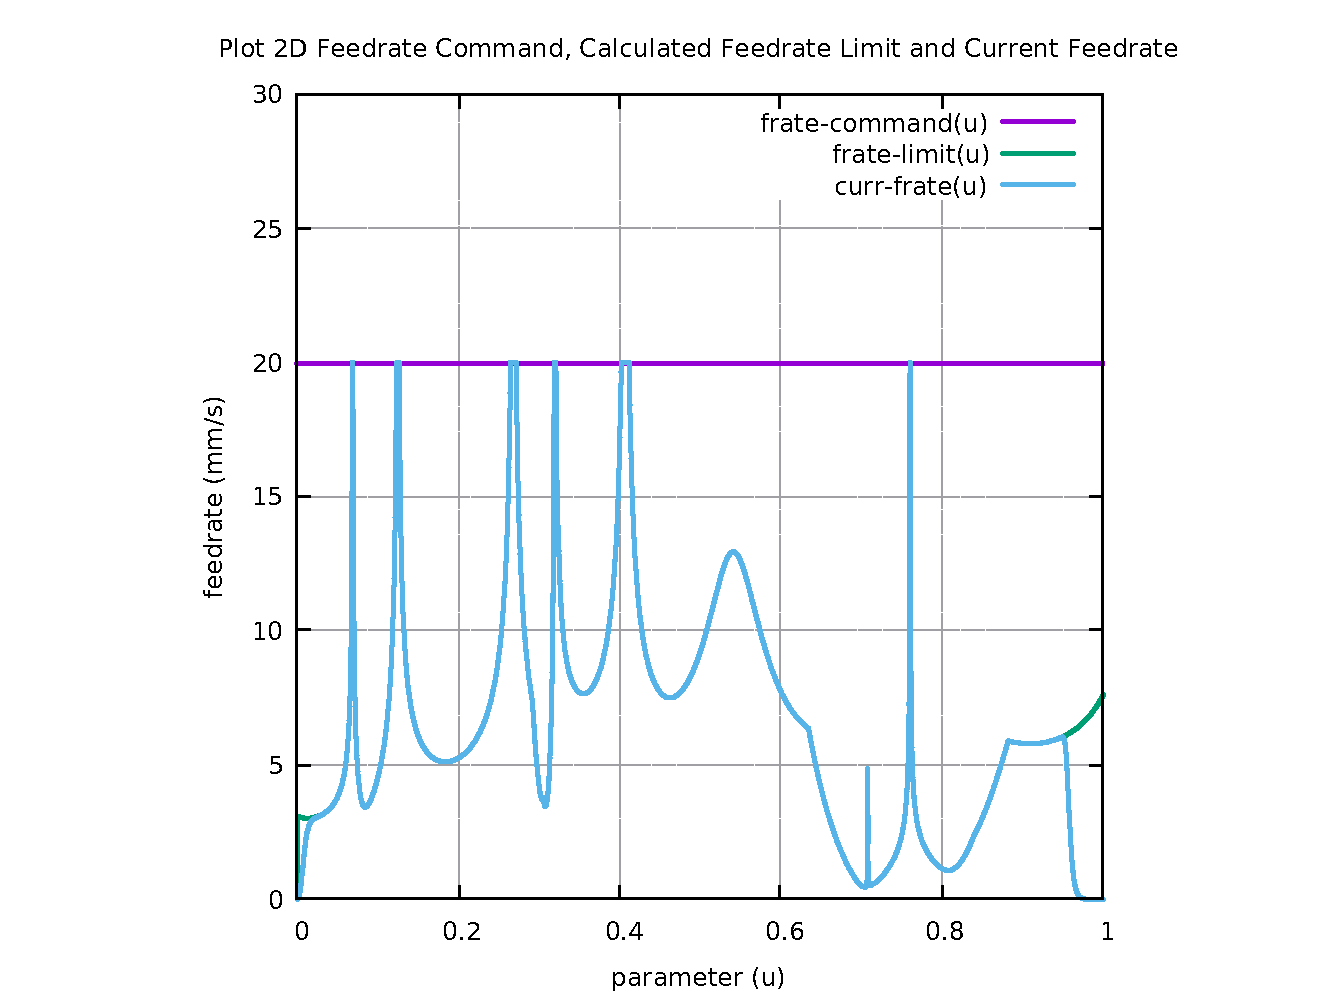
\includegraphics[width=1.00\textwidth]{Chap4/appendix/app-SnaHyp/plots/11-img-SnaHyp-FrateCommand-FrateLimit-and-Curr-Frate.pdf}
\end{figure}

\begin{figure}
	\caption     {SnaHyp FeedRateLimit minus CurrFeedRate}
	\label{12-img-SnaHyp-FeedRateLimit-minus-CurrFeedRate.pdf}
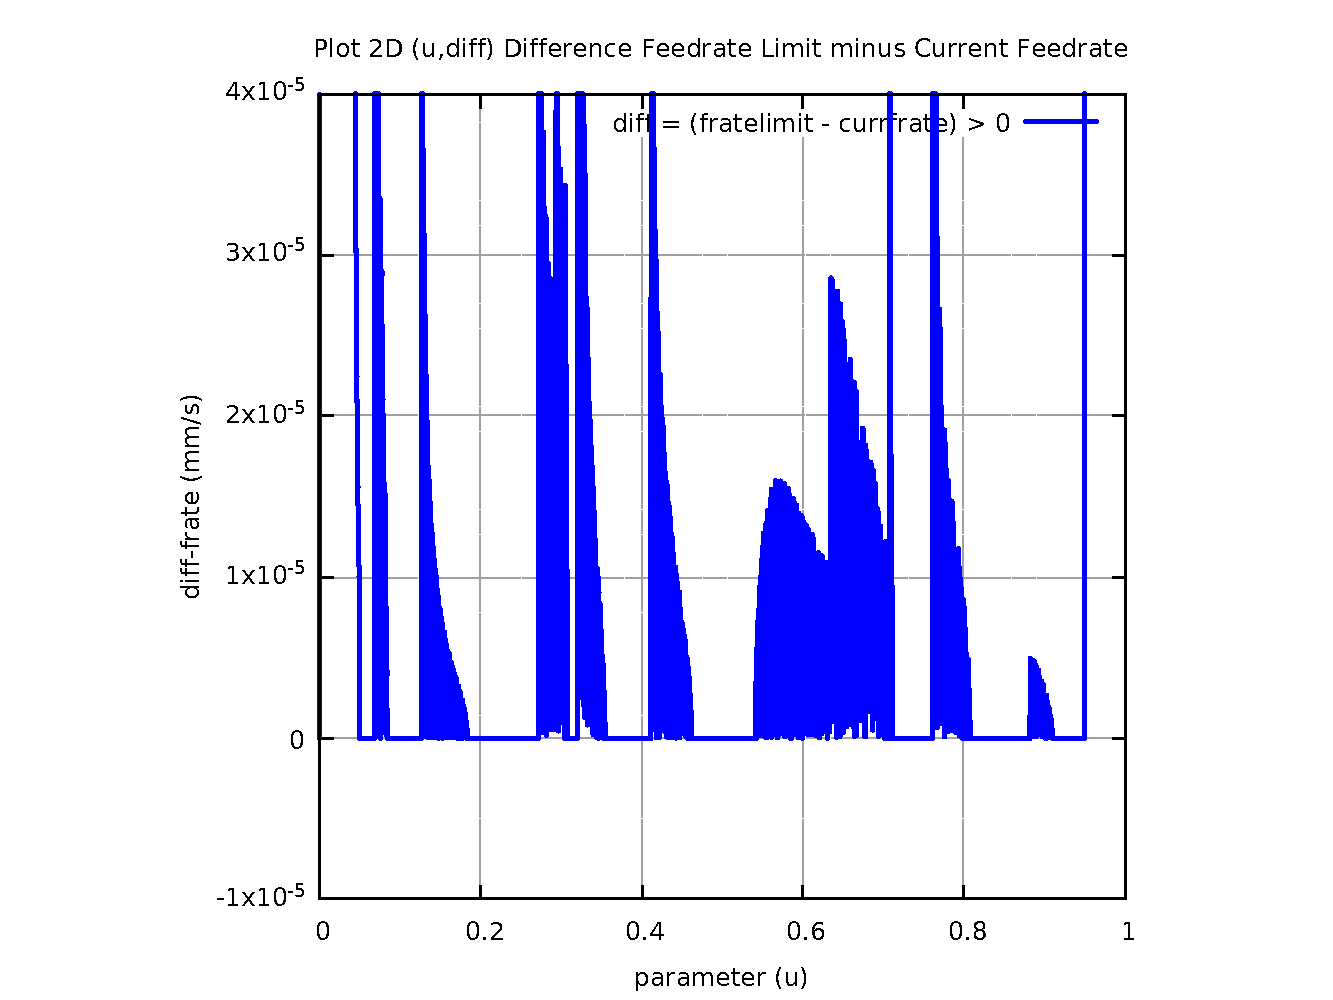
\includegraphics[width=1.00\textwidth]{Chap4/appendix/app-SnaHyp/plots/12-img-SnaHyp-FeedRateLimit-minus-CurrFeedRate.pdf}
\end{figure}

%% ==================================================
\clearpage
\pagebreak

\begin{figure}
	\caption     {SnaHyp FC20-Nominal X and Y Feedrate Profiles}
	\label{13-img-SnaHyp-FC20-Nominal-X-and-Y-Feedrate-Profiles.pdf}
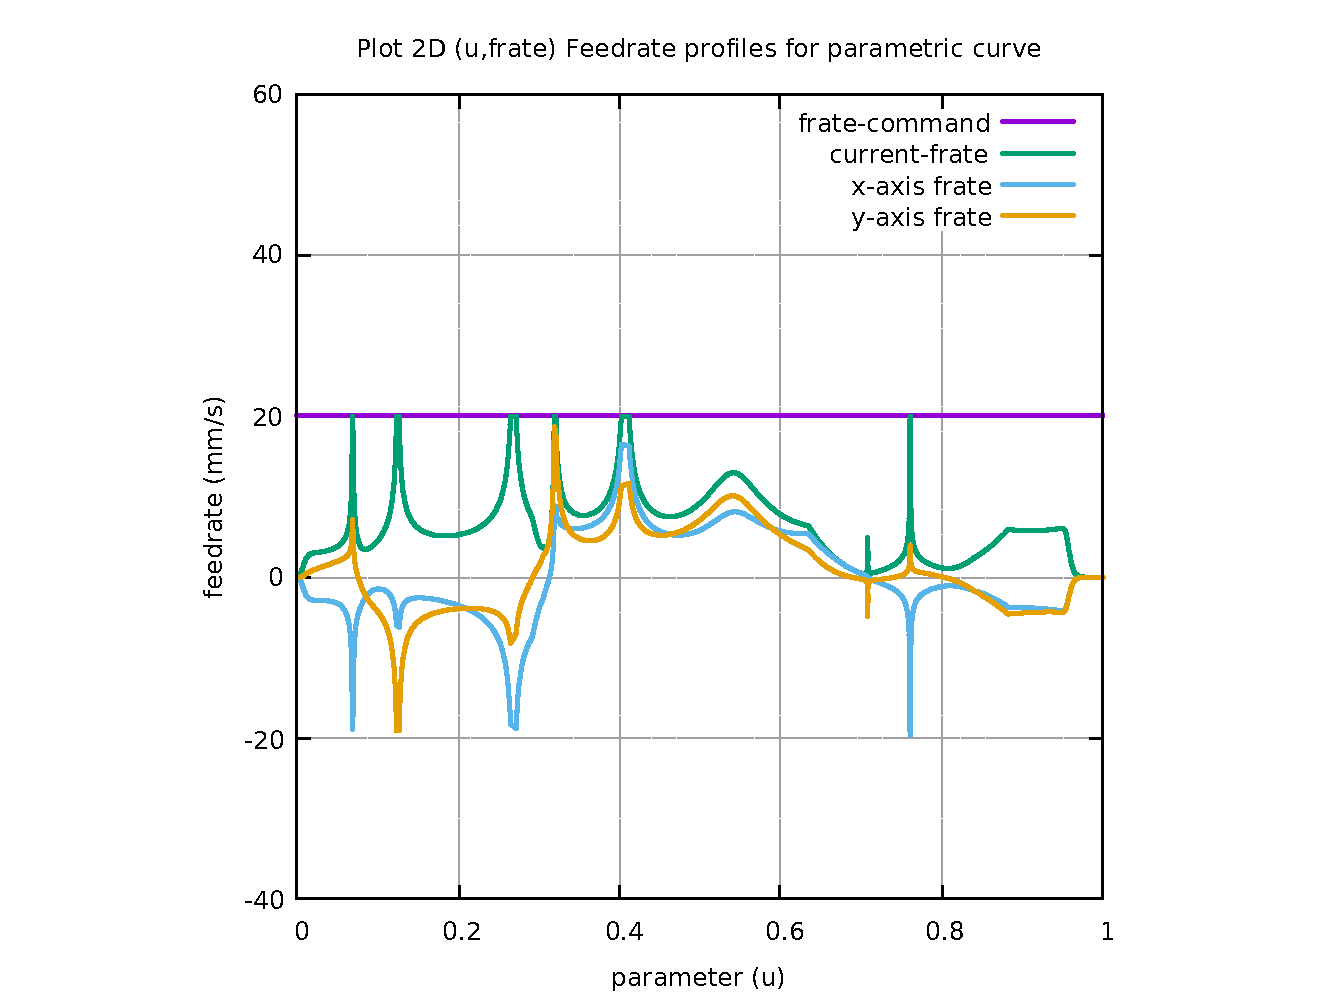
\includegraphics[width=1.00\textwidth]{Chap4/appendix/app-SnaHyp/plots/13-img-SnaHyp-FC20-Nominal-X-and-Y-Feedrate-Profiles.pdf}
\end{figure}


\begin{figure}
	\caption     {SnaHyp FC20 Nominal Tangential Acceleration}
	\label{14-img-SnaHyp-FC20-Nominal-Tangential-Acceleration.pdf}
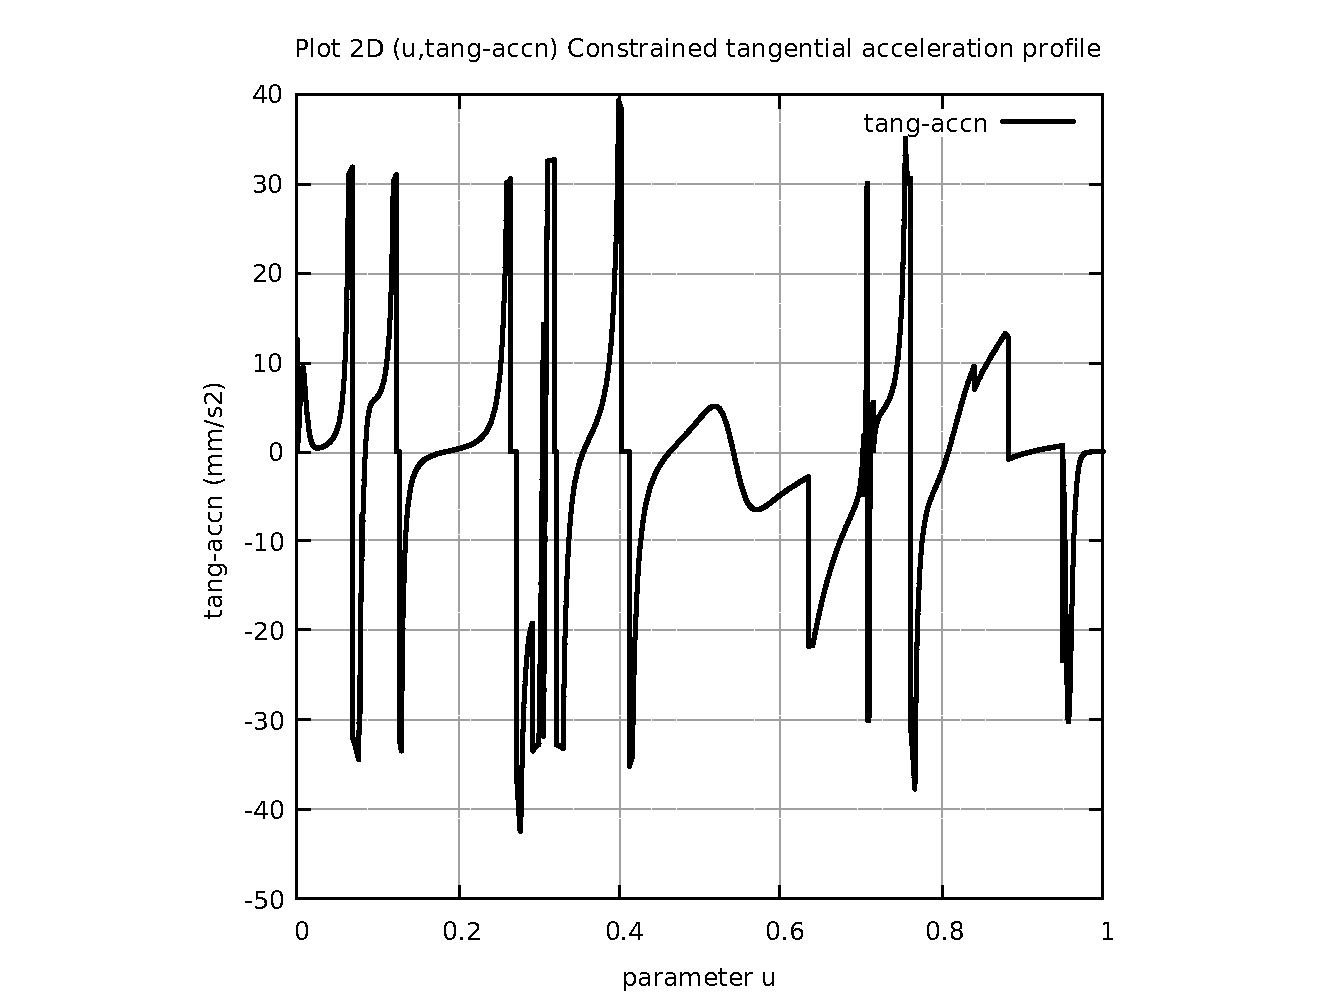
\includegraphics[width=1.00\textwidth]{Chap4/appendix/app-SnaHyp/plots/14-img-SnaHyp-FC20-Nominal-Tangential-Acceleration.pdf}
\end{figure}

%% ==================================================
\clearpage
\pagebreak

\begin{figure}
	\caption     {SnaHyp FC20 Nominal Rising S-Curve Profile}
	\label{15-img-SnaHyp-FC20-Nominal-Rising-S-Curve-Profile.pdf}
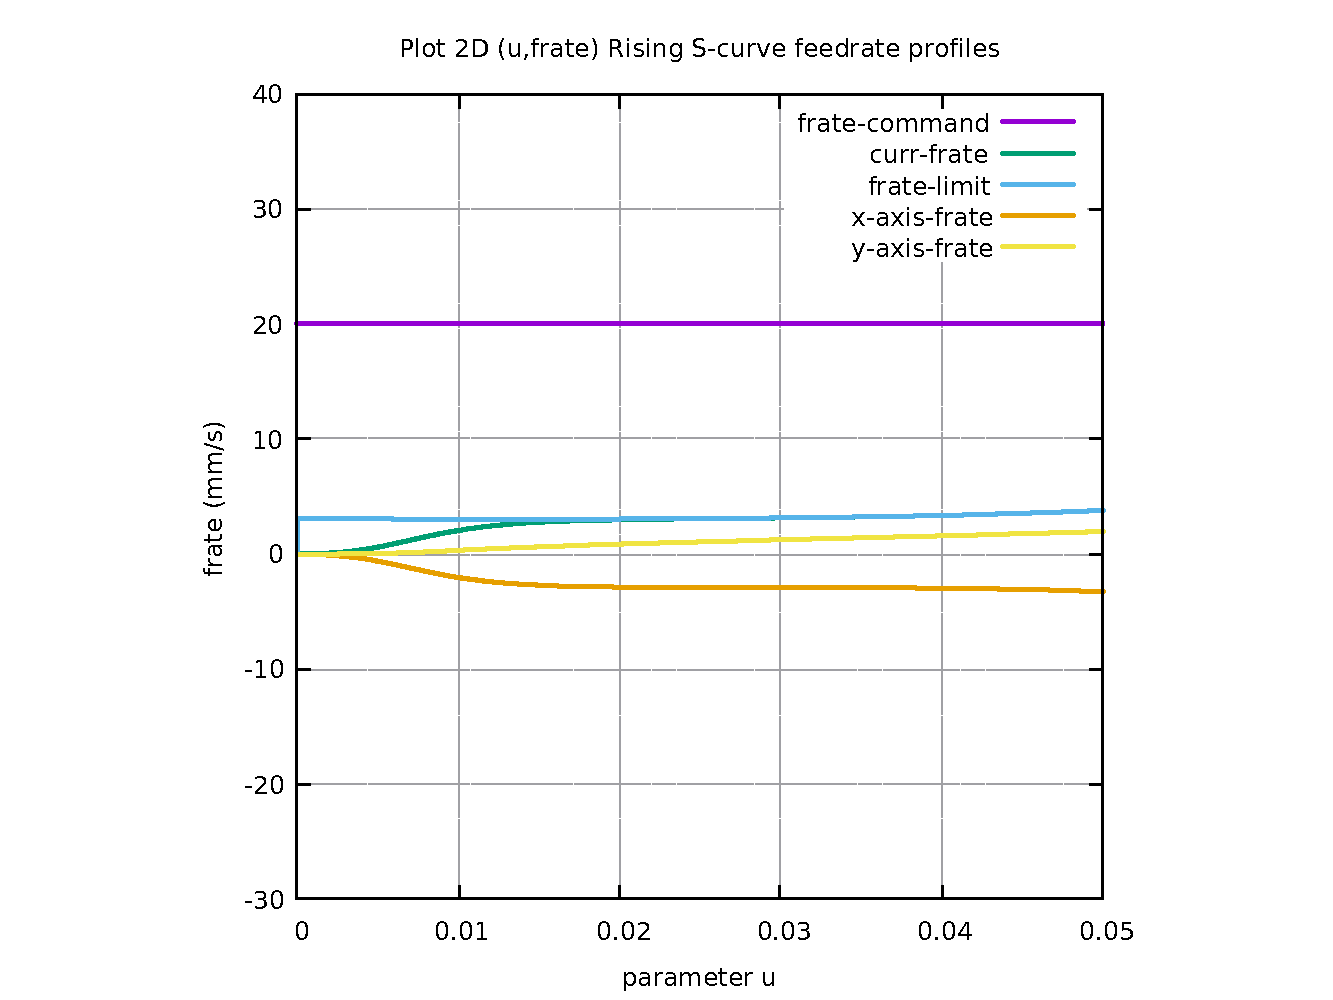
\includegraphics[width=1.00\textwidth]{Chap4/appendix/app-SnaHyp/plots/15-img-SnaHyp-FC20-Nominal-Rising-S-Curve-Profile.pdf}
\end{figure}


\begin{figure}
	\caption     {SnaHyp FC20 Nominal Falling S-Curve Profile}
	\label{16-img-SnaHyp-FC20-Nominal-Falling-S-Curve-Profile.pdf}
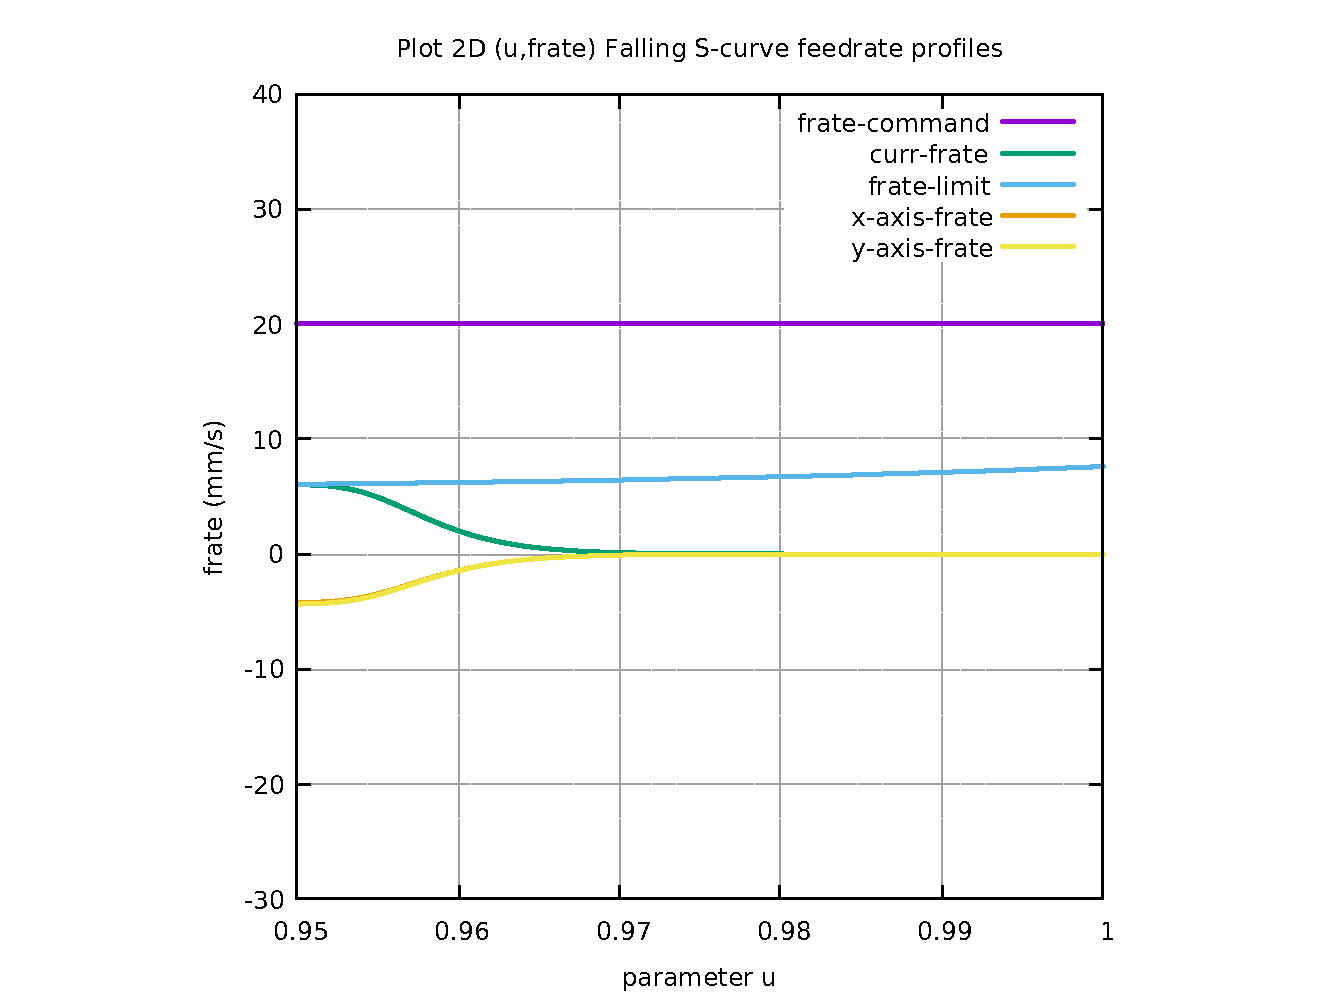
\includegraphics[width=1.00\textwidth]{Chap4/appendix/app-SnaHyp/plots/16-img-SnaHyp-FC20-Nominal-Falling-S-Curve-Profile.pdf}
\end{figure}

%% ==================================================
\clearpage
\pagebreak

\begin{figure}
	\caption     {SnaHyp FC10 Colored Feedrate Profile data ngcode}
	\label{17-img-SnaHyp-FC10-Colored-Feedrate-Profile-data_ngcode.png}
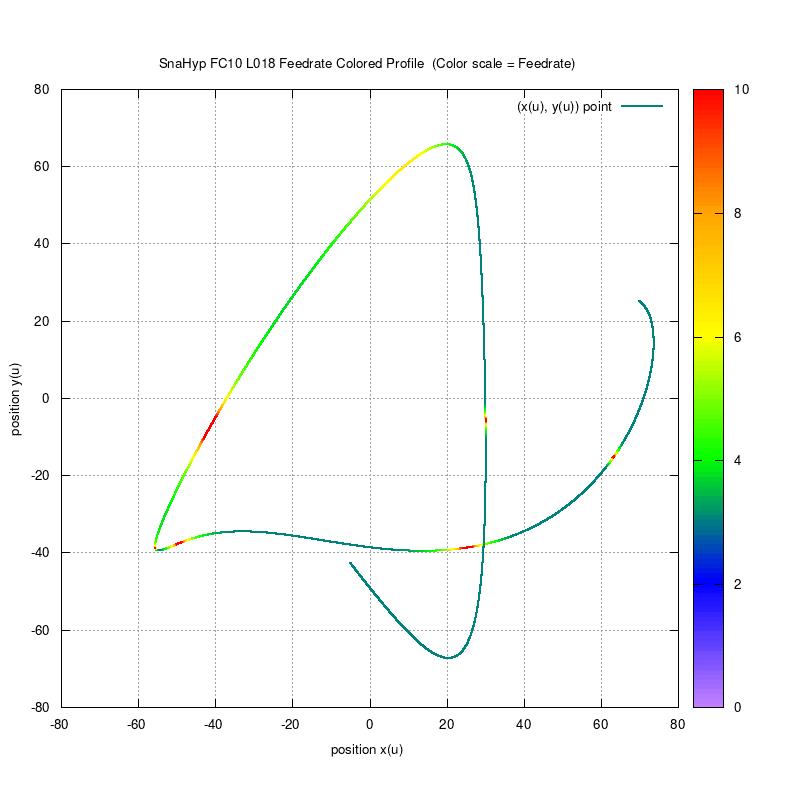
\includegraphics[width=0.75\textwidth]{Chap4/appendix/app-SnaHyp/plots/17-img-SnaHyp-FC10-Colored-Feedrate-Profile-data_ngcode.png}
\end{figure}


\begin{figure}
	\caption     {SnaHyp FC20 Colored Feedrate Profile data ngcode}
	\label{18-img-SnaHyp-FC20-Colored-Feedrate-Profile-data_ngcode.png}
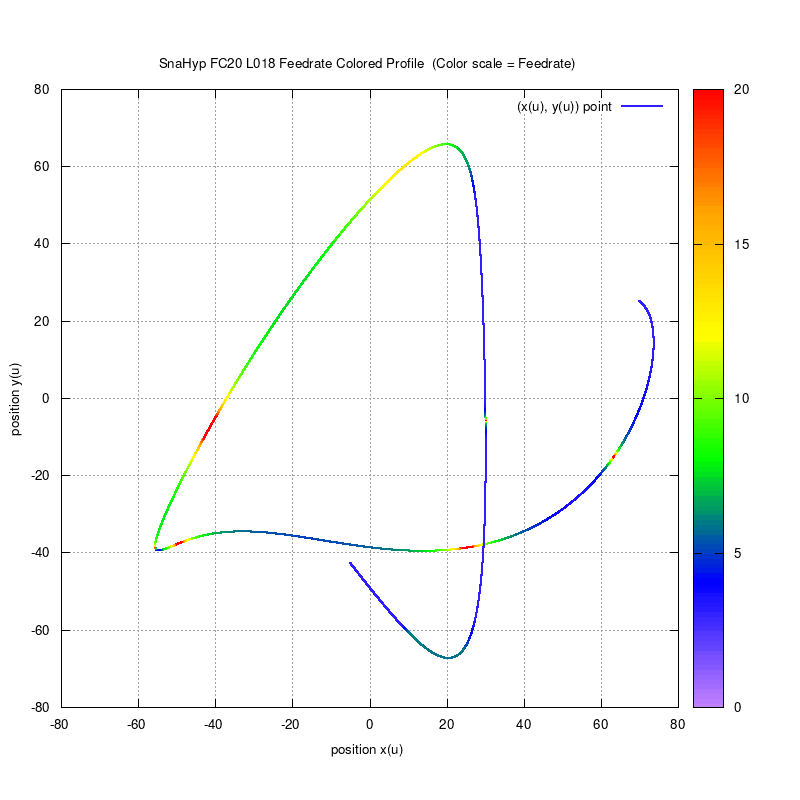
\includegraphics[width=0.75\textwidth]{Chap4/appendix/app-SnaHyp/plots/18-img-SnaHyp-FC20-Colored-Feedrate-Profile-data_ngcode.png}
\end{figure}

%% ==================================================
\clearpage
\pagebreak

\begin{figure}
	\caption     {SnaHyp FC25 Colored Feedrate Profile data ngcode}
	\label{19-img-SnaHyp-FC25-Colored-Feedrate-Profile-data_ngcode.png}
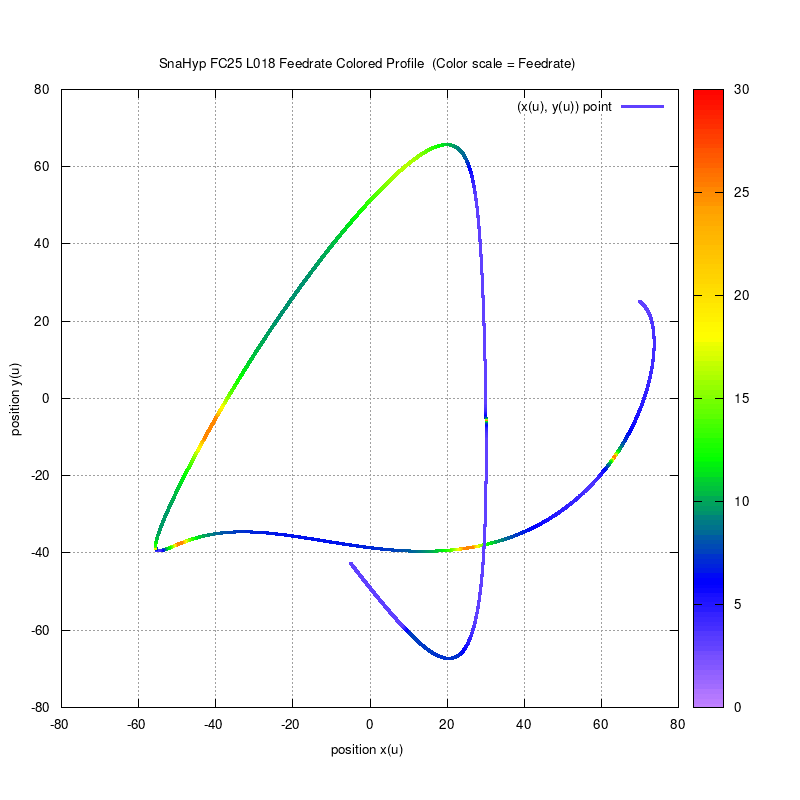
\includegraphics[width=0.75\textwidth]{Chap4/appendix/app-SnaHyp/plots/19-img-SnaHyp-FC25-Colored-Feedrate-Profile-data_ngcode.png}
\end{figure}


\begin{figure}
	\caption     {SnaHyp FC28 Colored Feedrate Profile data ngcode}
	\label{20-img-SnaHyp-FC28-Colored-Feedrate-Profile-data_ngcode.png}
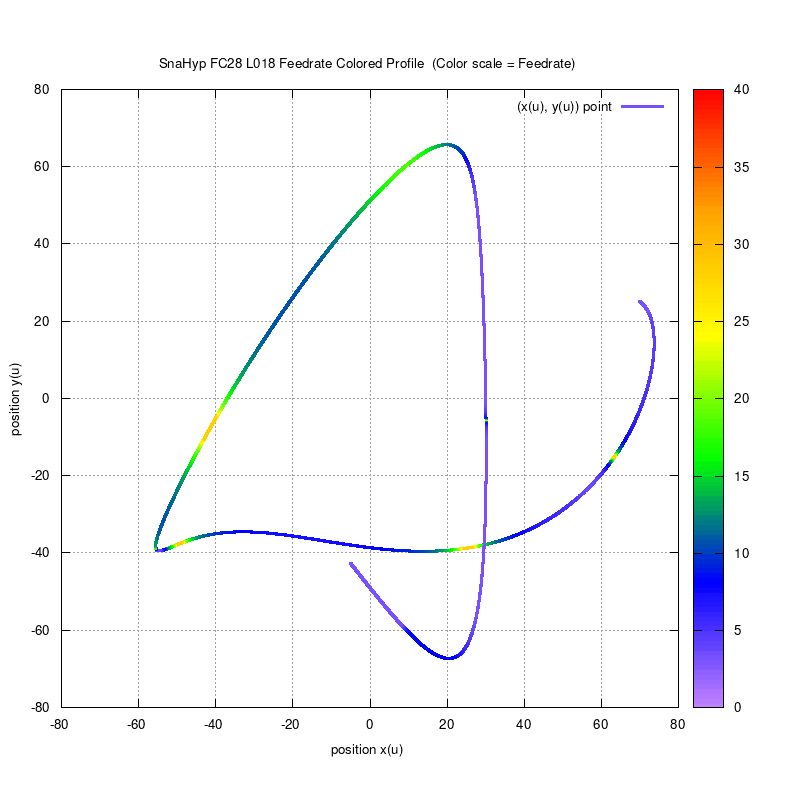
\includegraphics[width=0.75\textwidth]{Chap4/appendix/app-SnaHyp/plots/20-img-SnaHyp-FC28-Colored-Feedrate-Profile-data_ngcode.png}
\end{figure}

%% ==================================================
\clearpage
\pagebreak

\begin{figure}
	\caption     {SnaHyp FC10 Tangential Acceleration}
	\label{21-img-SnaHyp-FC10-Tangential-Acceleration.pdf}
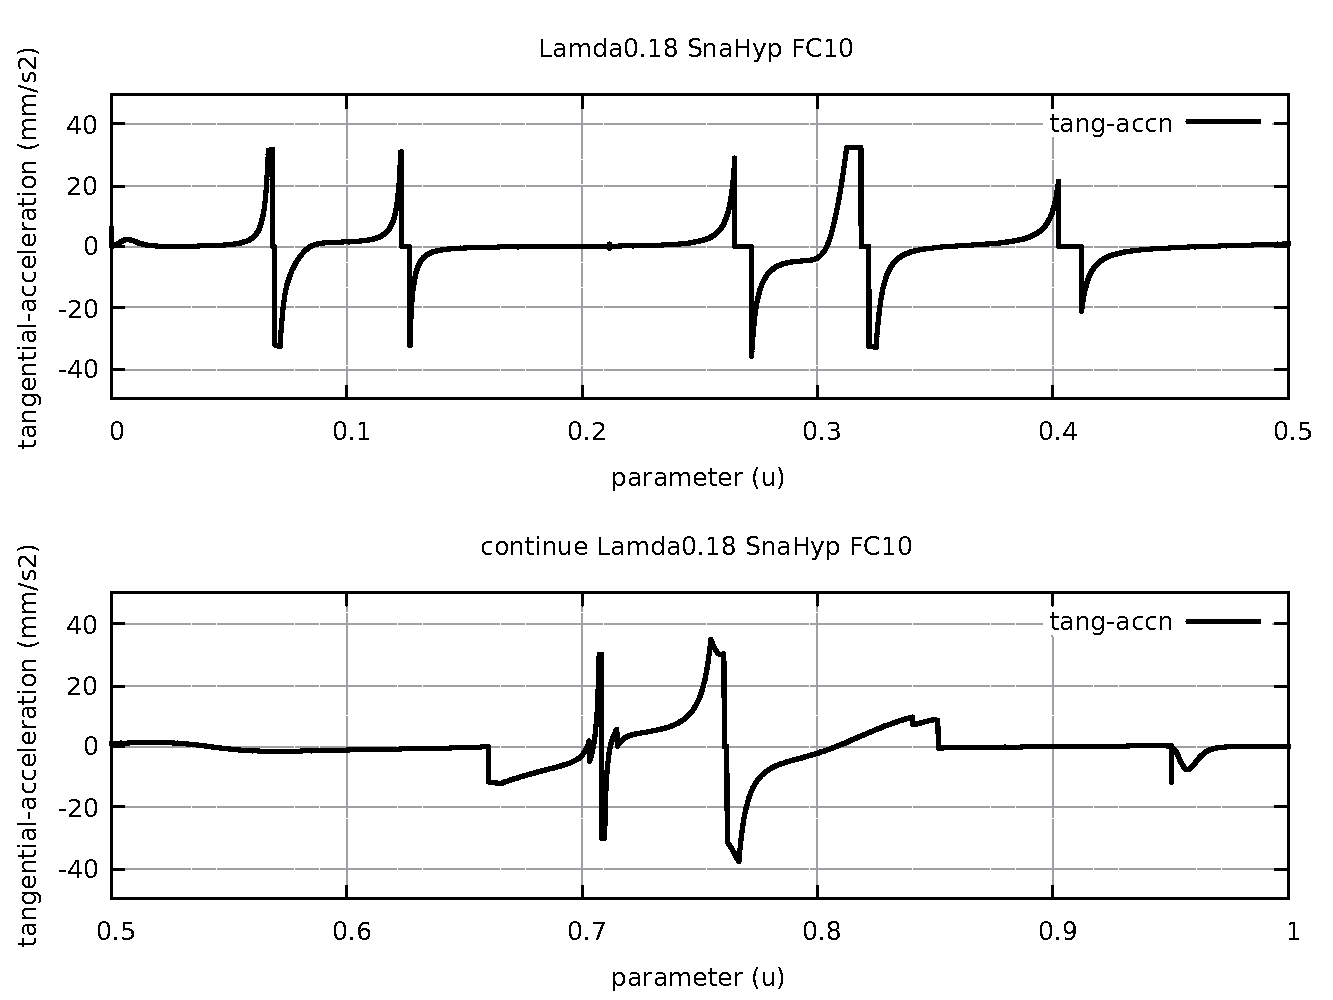
\includegraphics[width=1.00\textwidth]{Chap4/appendix/app-SnaHyp/plots/21-img-SnaHyp-FC10-Tangential-Acceleration.pdf}
\end{figure}


\begin{figure}
	\caption     {SnaHyp FC20 Tangential Acceleration}
	\label{22-img-SnaHyp-FC20-Tangential-Acceleration.pdf}
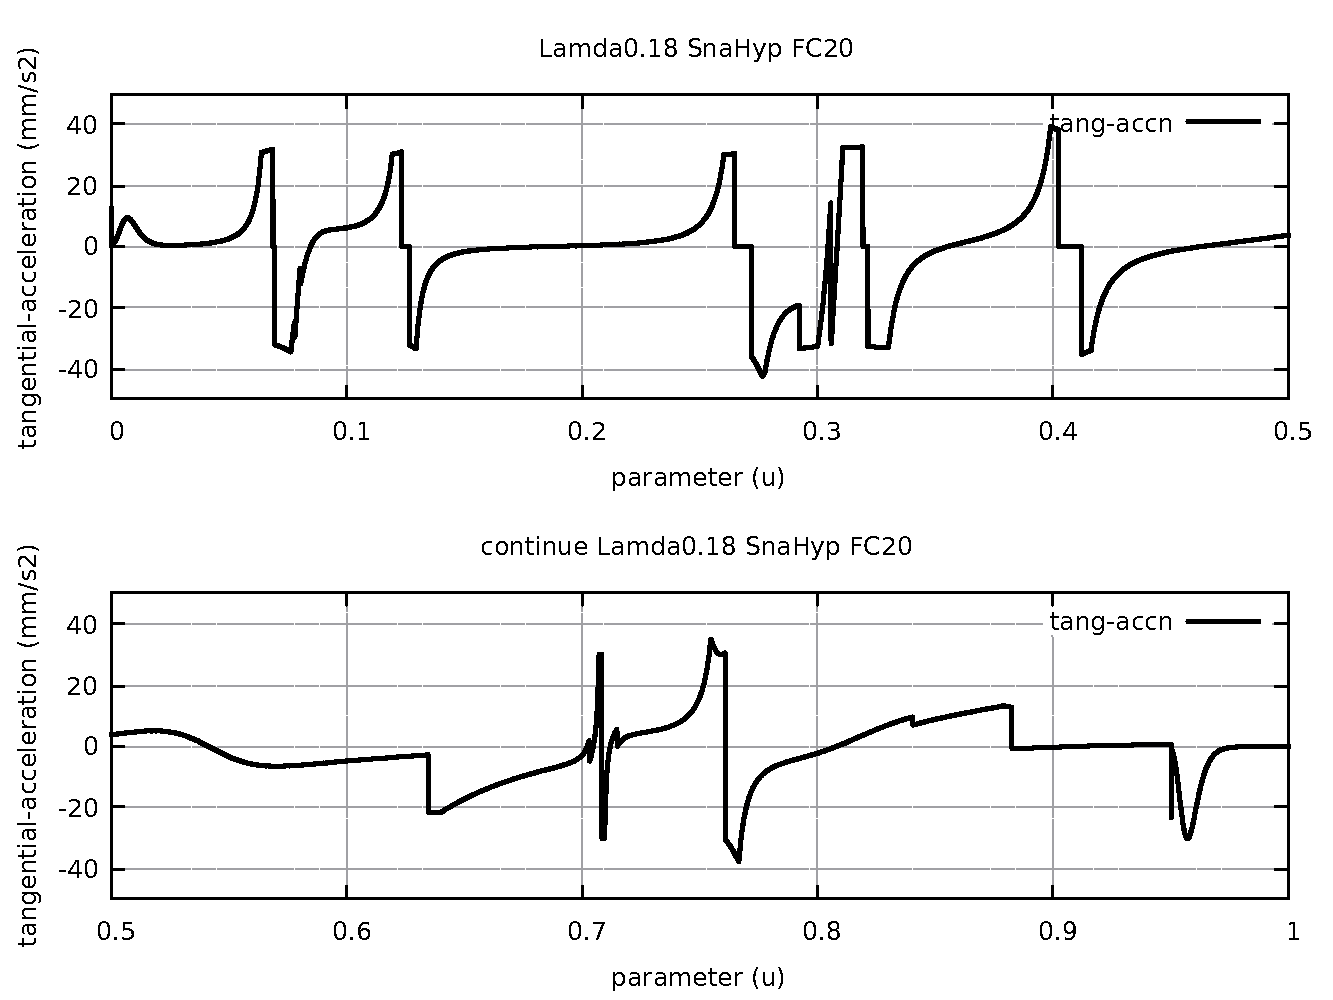
\includegraphics[width=1.00\textwidth]{Chap4/appendix/app-SnaHyp/plots/22-img-SnaHyp-FC20-Tangential-Acceleration.pdf}
\end{figure}

%% ==================================================
\clearpage
\pagebreak

\begin{figure}
	\caption     {SnaHyp FC30 Tangential Acceleration}
	\label{23-img-SnaHyp-FC30-Tangential-Acceleration.pdf}
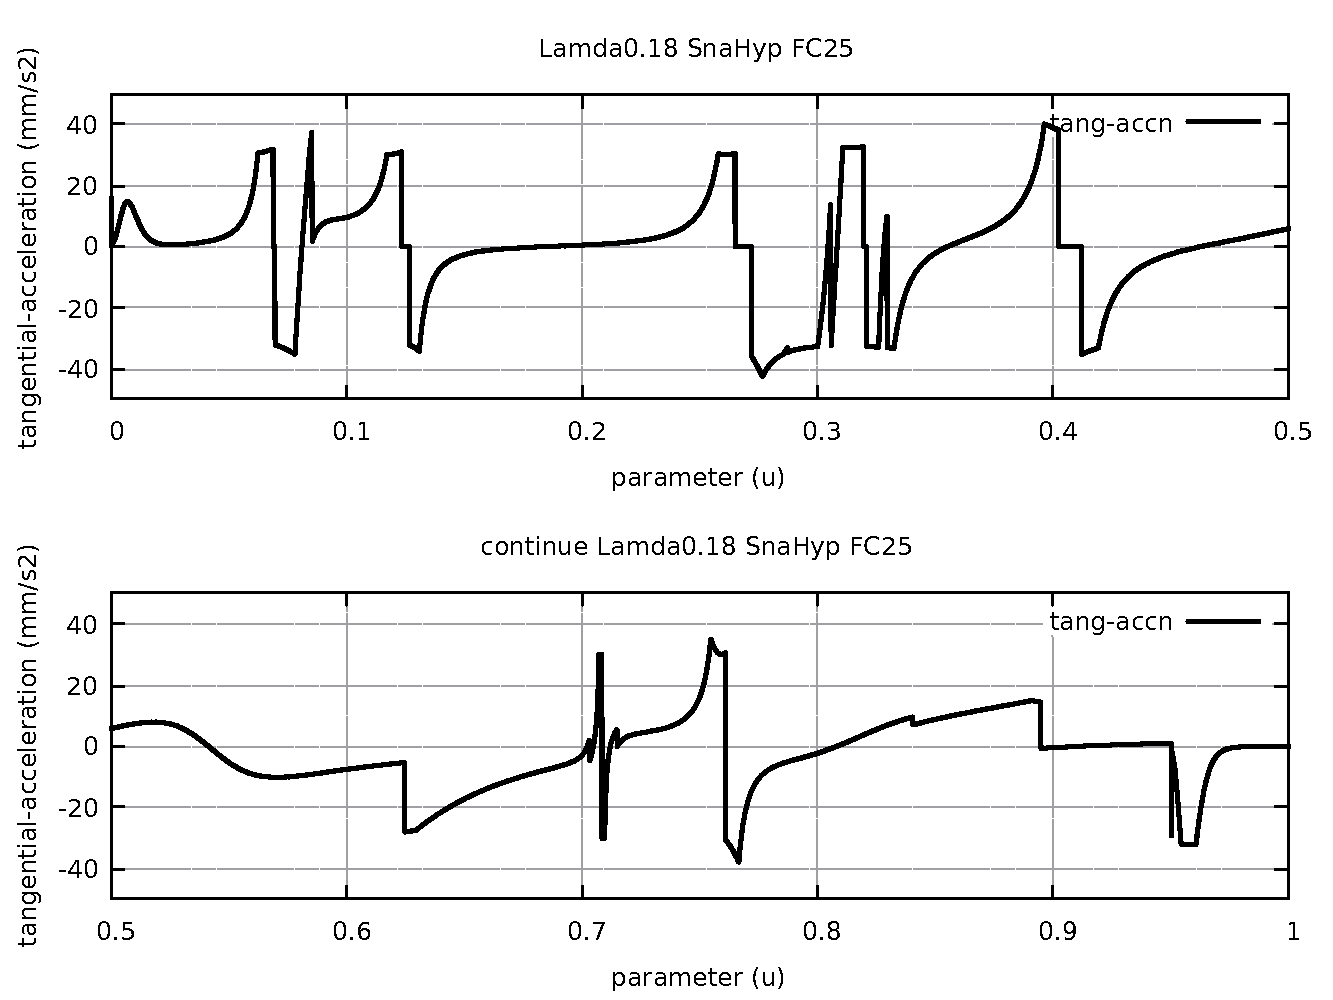
\includegraphics[width=1.00\textwidth]{Chap4/appendix/app-SnaHyp/plots/23-img-SnaHyp-FC30-Tangential-Acceleration.pdf}
\end{figure}


\begin{figure}
	\caption     {SnaHyp FC40 Tangential Acceleration}
	\label{24-img-SnaHyp-FC40-Tangential-Acceleration.pdf}
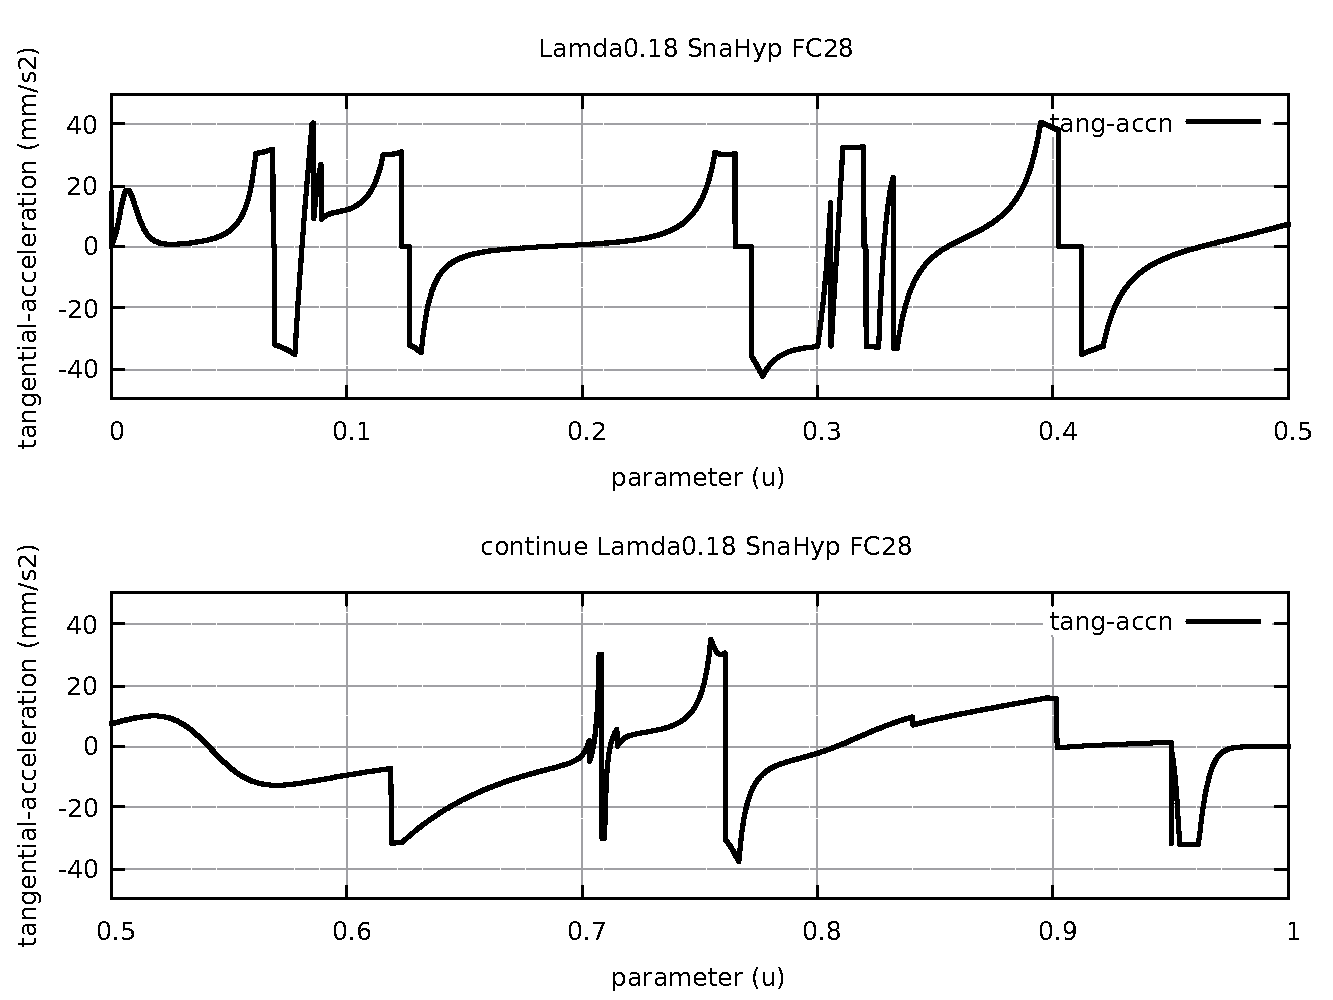
\includegraphics[width=1.00\textwidth]{Chap4/appendix/app-SnaHyp/plots/24-img-SnaHyp-FC40-Tangential-Acceleration.pdf}
\end{figure}

%% ==================================================
\clearpage
\pagebreak

\begin{figure}
	\caption     {SnaHyp FC20 Nominal Separation NAL and NCL}
	\label{25-img-SnaHyp-FC20-Nominal-Separation-NAL-and-NCL.pdf}
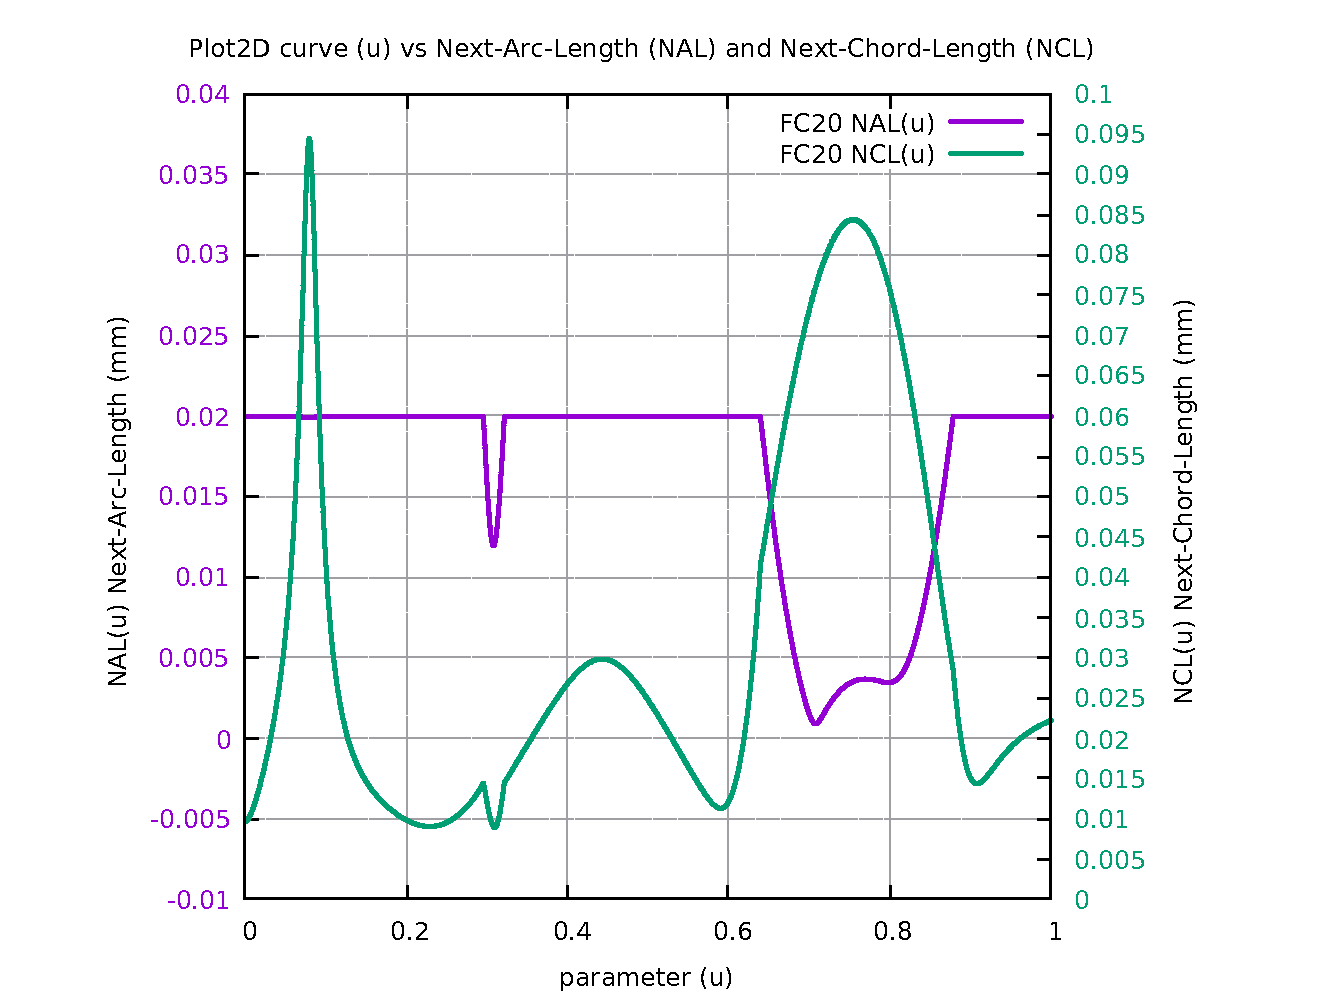
\includegraphics[width=1.00\textwidth]{Chap4/appendix/app-SnaHyp/plots/25-img-SnaHyp-FC20-Nominal-Separation-NAL-and-NCL.pdf}
\end{figure}


\begin{figure}
	\caption     {SnaHyp Difference SAL minus SCL for FC10 FC20 FC30 FC40}
	\label{26-img-SnaHyp-Difference-SAL-minus-SCL-for-FC10-FC20-FC30-FC40.pdf}
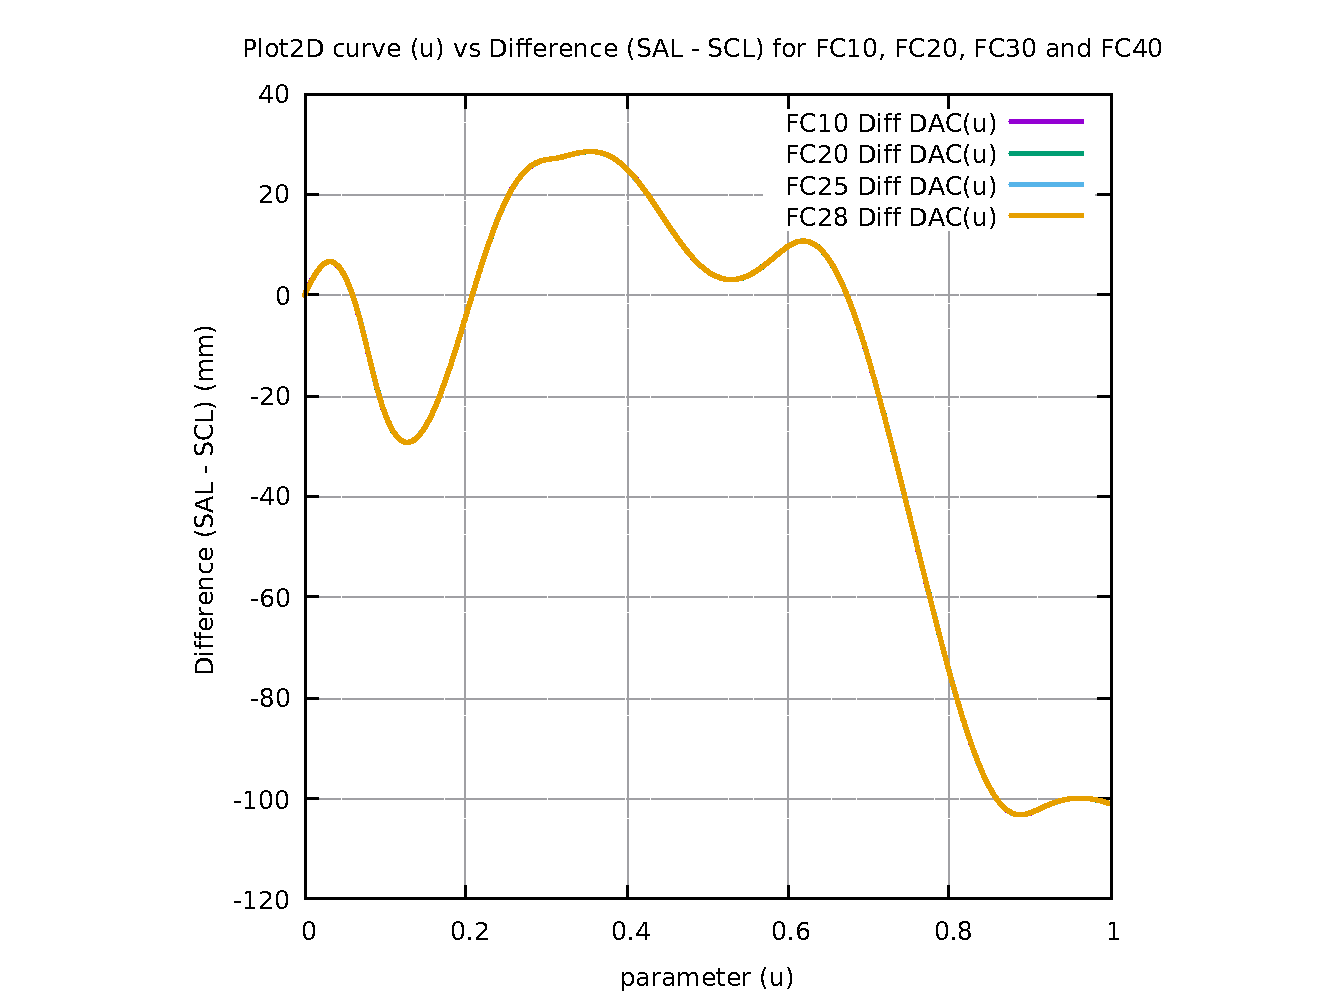
\includegraphics[width=1.00\textwidth]{Chap4/appendix/app-SnaHyp/plots/26-img-SnaHyp-Difference-SAL-minus-SCL-for-FC10-FC20-FC30-FC40.pdf}
\end{figure}


%% ==================================================
\clearpage
\pagebreak

\begin{figure}
	\caption     {SnaHyp FC10 FrateCmd CurrFrate X-Frate Y-Frate}
	\label{27-img-SnaHyp-FC10-FrateCmd-CurrFrate-X-Frate-Y-Frate.pdf}
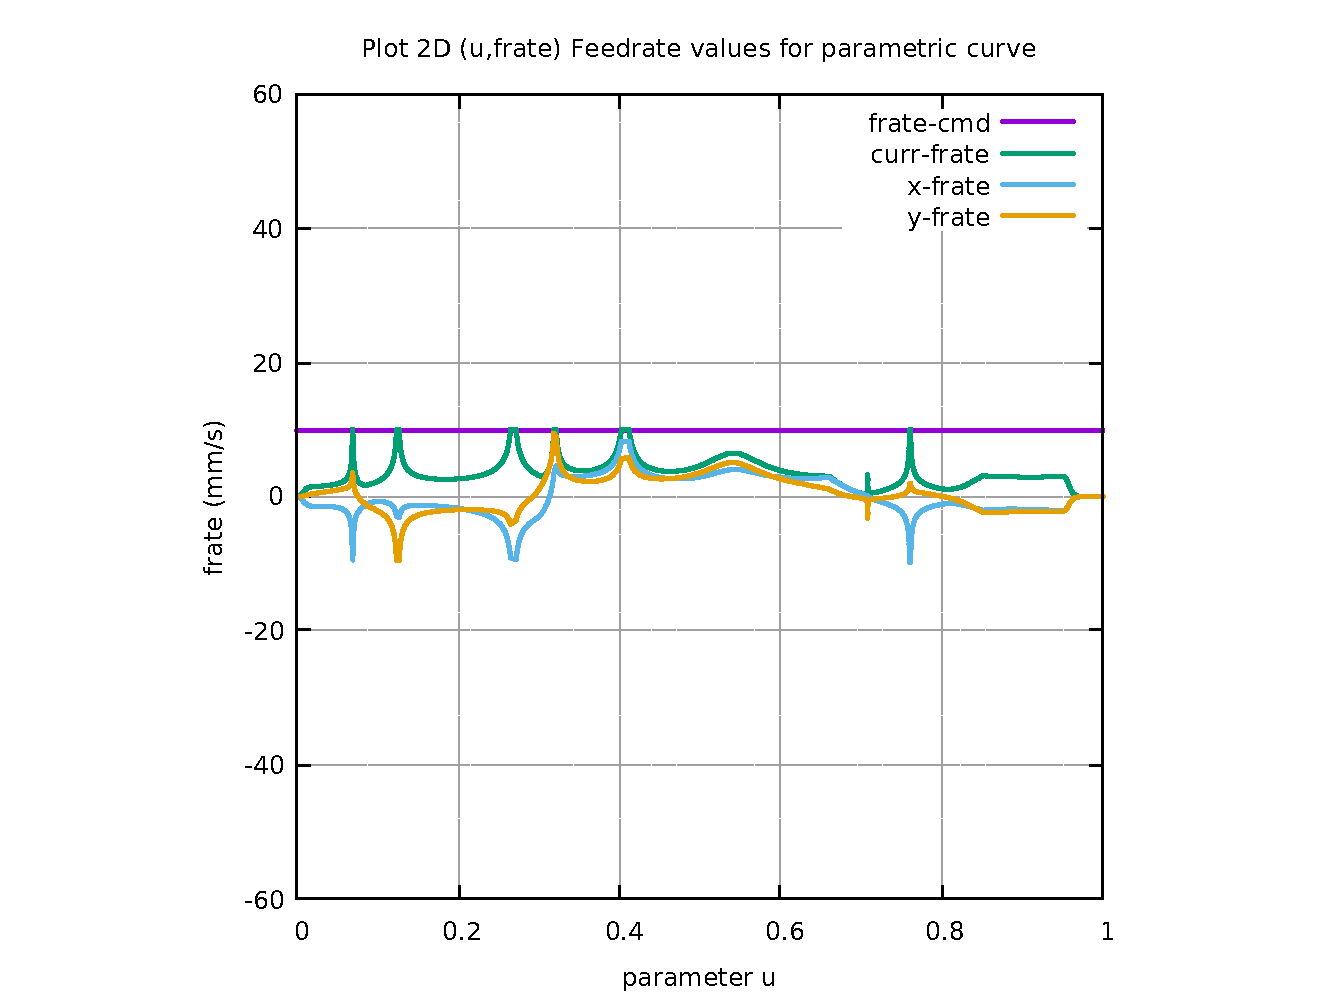
\includegraphics[width=1.00\textwidth]{Chap4/appendix/app-SnaHyp/plots/27-img-SnaHyp-FC10-FrateCmd-CurrFrate-X-Frate-Y-Frate.pdf}
\end{figure}


\begin{figure}
	\caption     {SnaHyp FC20 FrateCmd CurrFrate X-Frate Y-Frate}
	\label{28-img-SnaHyp-FC20-FrateCmd-CurrFrate-X-Frate-Y-Frate.pdf}
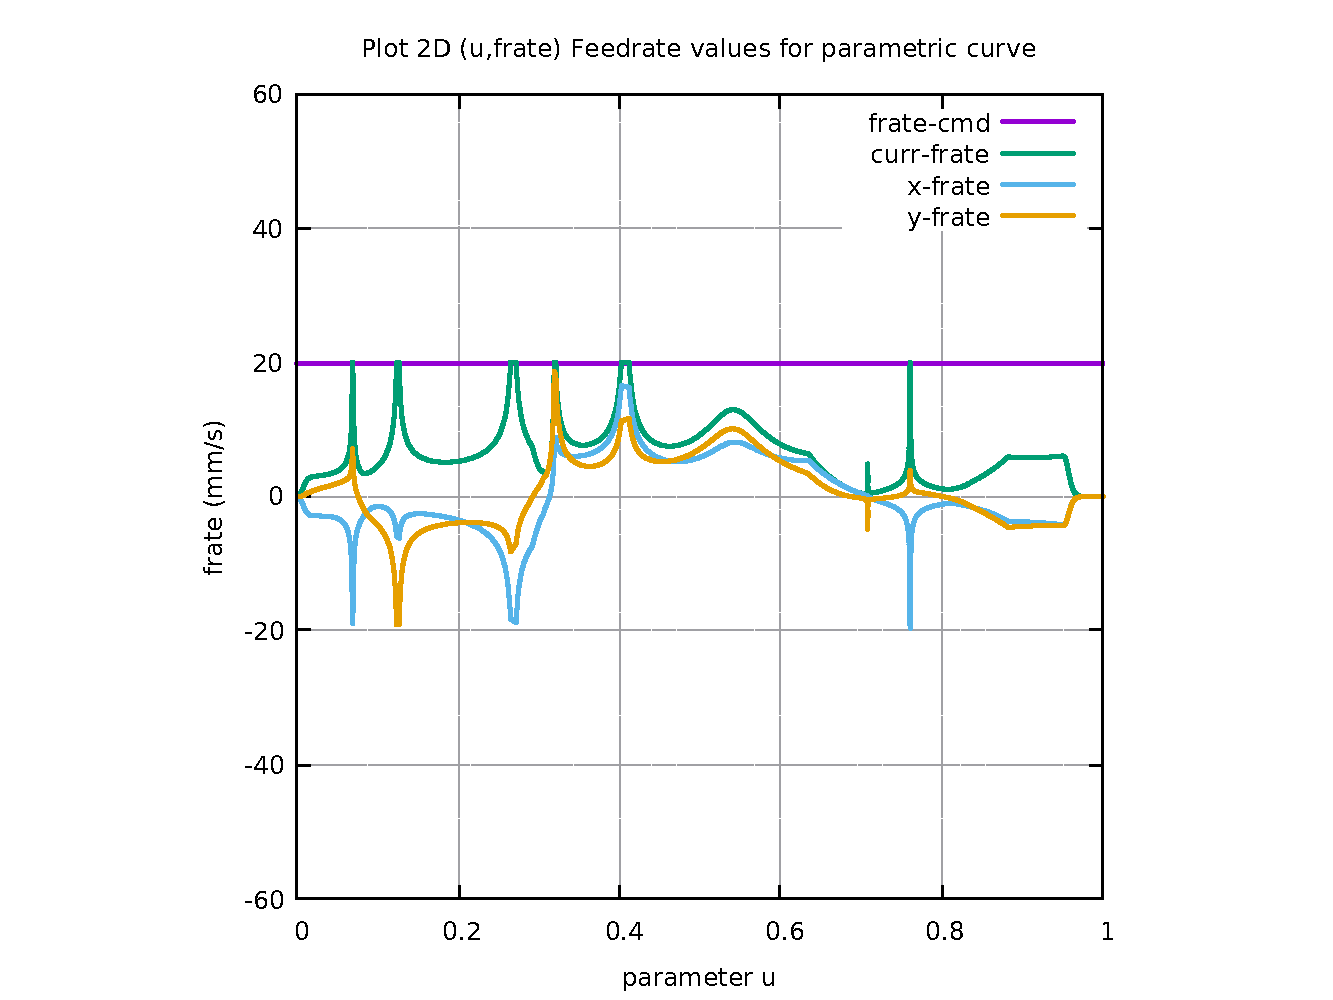
\includegraphics[width=1.00\textwidth]{Chap4/appendix/app-SnaHyp/plots/28-img-SnaHyp-FC20-FrateCmd-CurrFrate-X-Frate-Y-Frate.pdf}
\end{figure}


%% ==================================================
\clearpage
\pagebreak

\begin{figure}
	\caption     {SnaHyp FC25 FrateCmd CurrFrate X-Frate Y-Frate}
	\label{29-img-SnaHyp-FC25-FrateCmd-CurrFrate-X-Frate-Y-Frate.pdf}
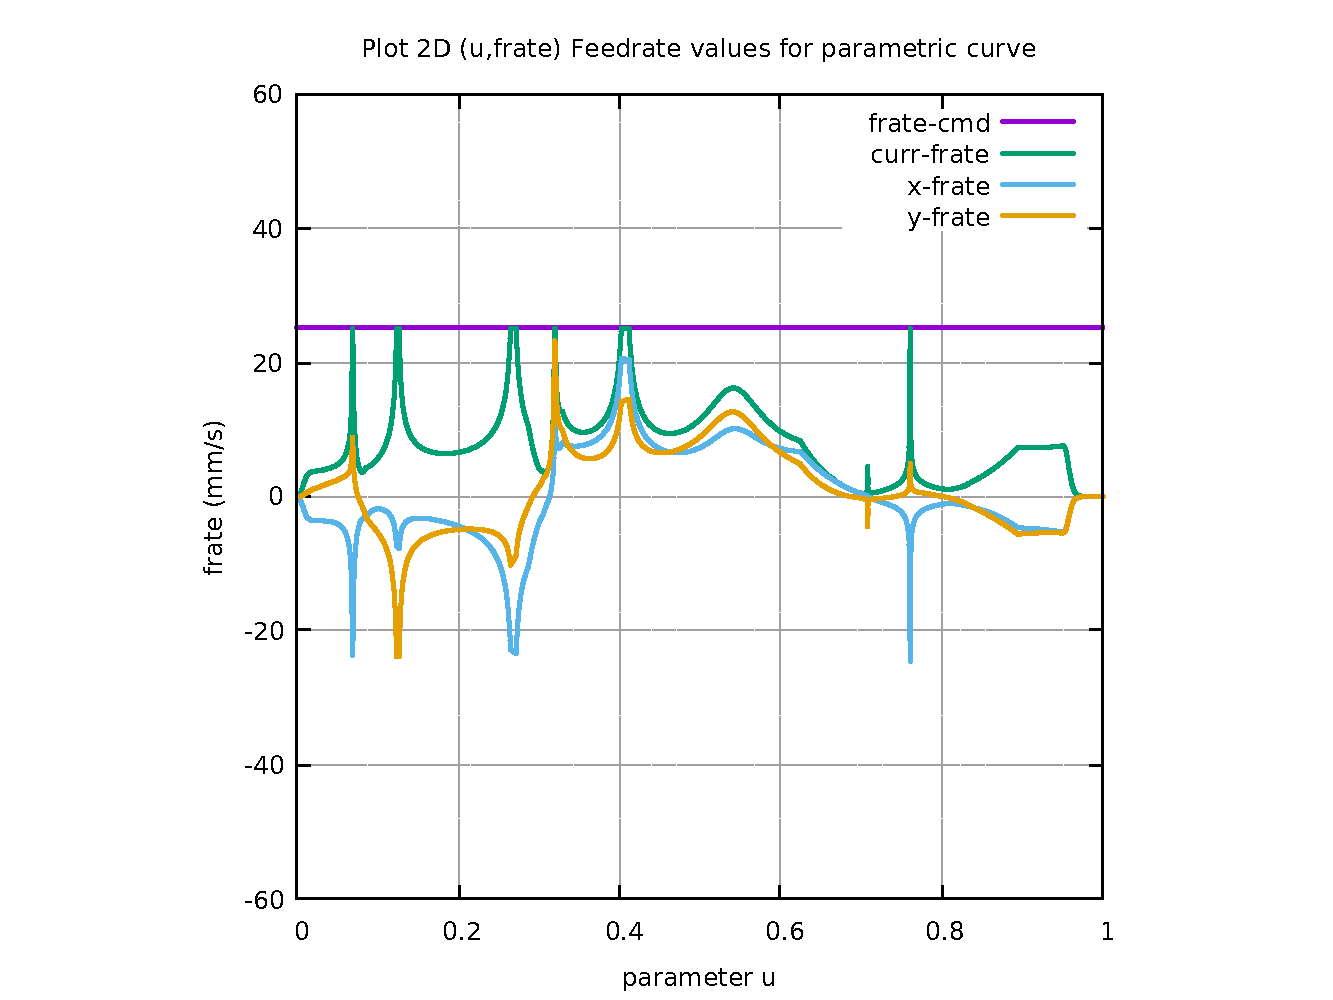
\includegraphics[width=1.00\textwidth]{Chap4/appendix/app-SnaHyp/plots/29-img-SnaHyp-FC30-FrateCmd-CurrFrate-X-Frate-Y-Frate.pdf}
\end{figure}


\begin{figure}
	\caption     {SnaHyp FC28 FrateCmd CurrFrate X-Frate Y-Frate}
	\label{30-img-SnaHyp-FC28-FrateCmd-CurrFrate-X-Frate-Y-Frate.pdf}
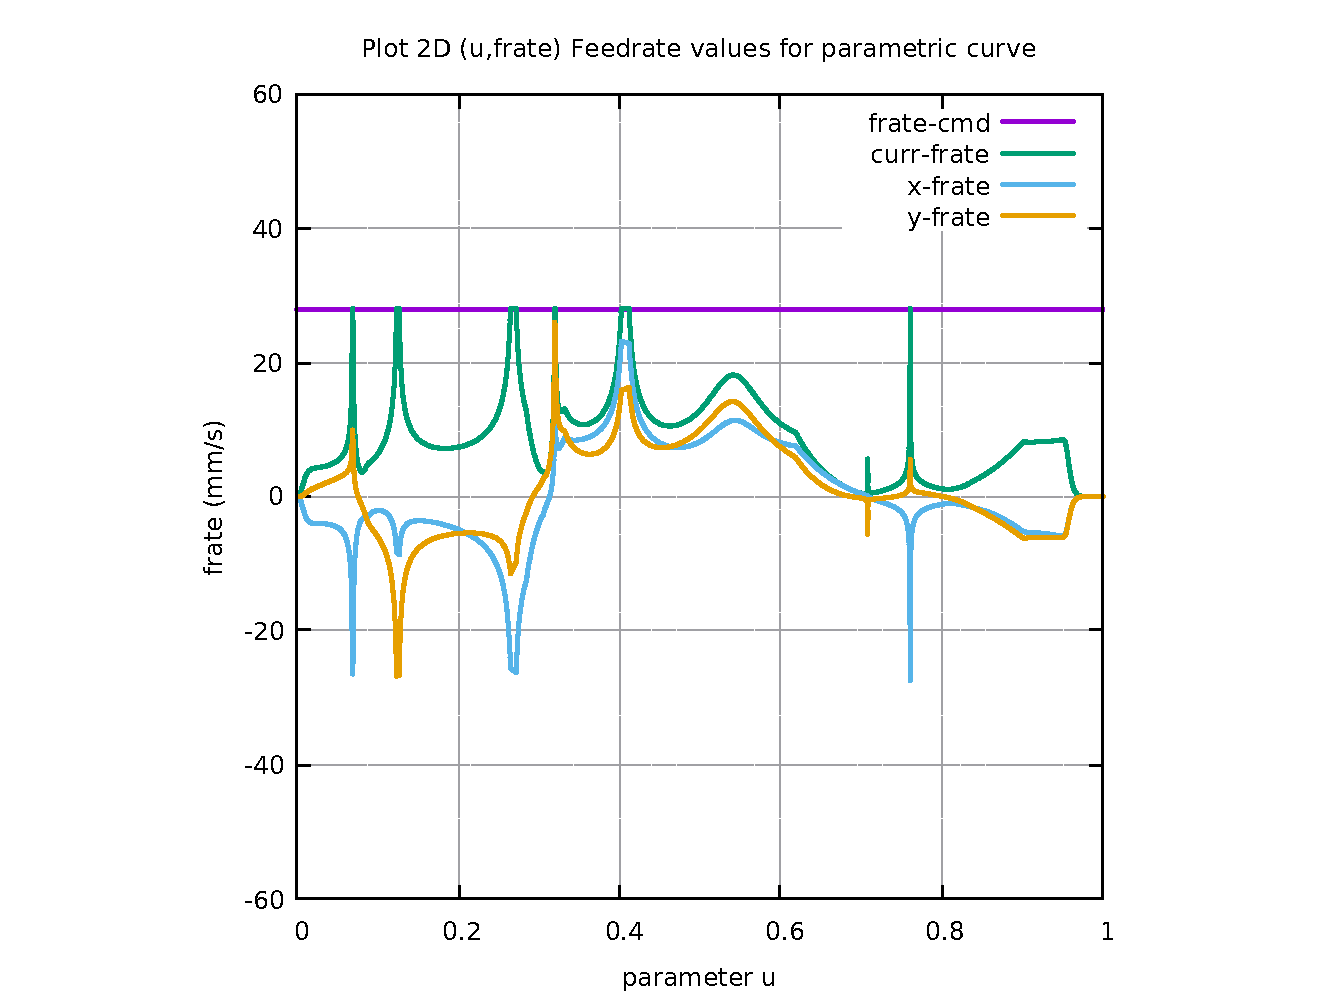
\includegraphics[width=1.00\textwidth]{Chap4/appendix/app-SnaHyp/plots/30-img-SnaHyp-FC40-FrateCmd-CurrFrate-X-Frate-Y-Frate.pdf}
\end{figure}


%% ==================================================
\clearpage
\pagebreak

\begin{figure}
	\caption     {SnaHyp FC10 Four Components FeedrateLimit}
	\label{31-img-SnaHyp-FC10-Four-Components-FeedrateLimit.pdf}
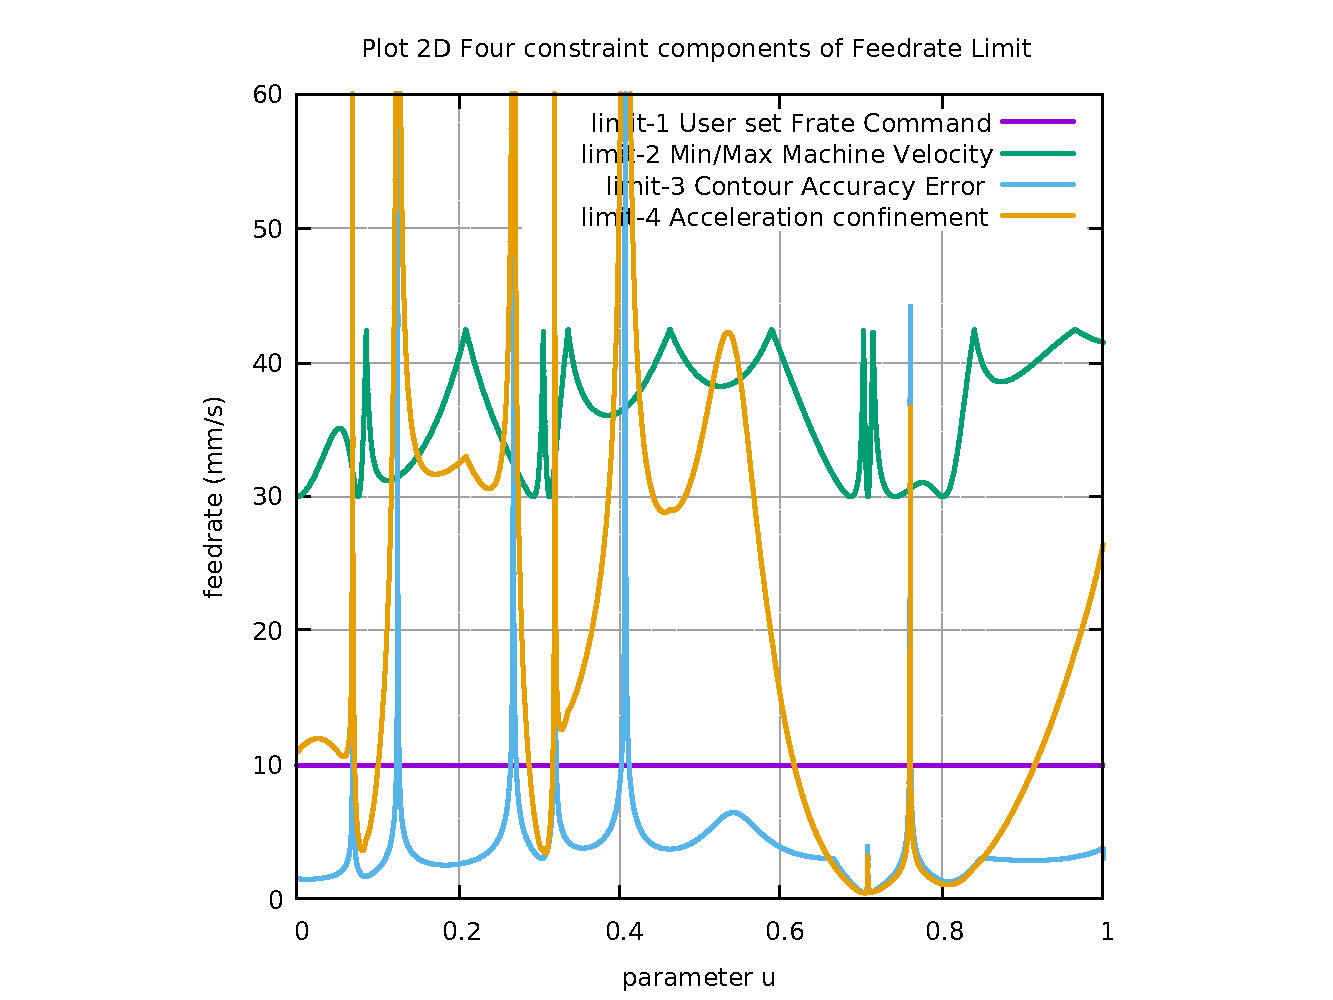
\includegraphics[width=1.00\textwidth]{Chap4/appendix/app-SnaHyp/plots/31-img-SnaHyp-FC10-Four-Components-FeedrateLimit.pdf}
\end{figure}


\begin{figure}
	\caption     {SnaHyp FC20 Four Components FeedrateLimit}
	\label{32-img-SnaHyp-FC20-Four-Components-FeedrateLimit.pdf}
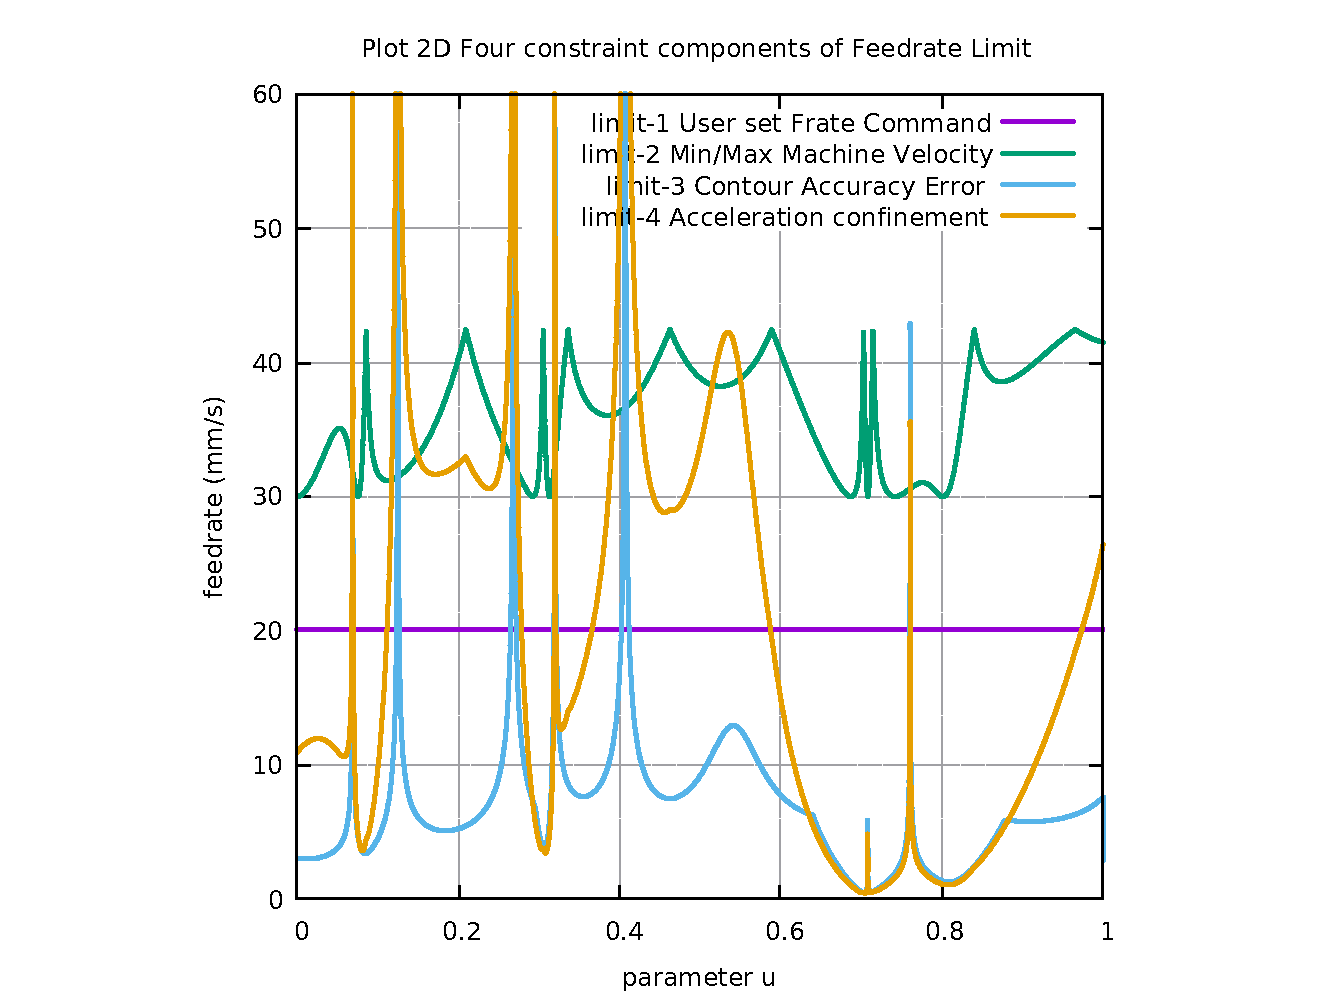
\includegraphics[width=1.00\textwidth]{Chap4/appendix/app-SnaHyp/plots/32-img-SnaHyp-FC20-Four-Components-FeedrateLimit.pdf}
\end{figure}


%% ==================================================
\clearpage
\pagebreak

\begin{figure}
	\caption     {SnaHyp FC25 Four Components FeedrateLimit}
	\label{33-img-SnaHyp-FC25-Four-Components-FeedrateLimit.pdf}
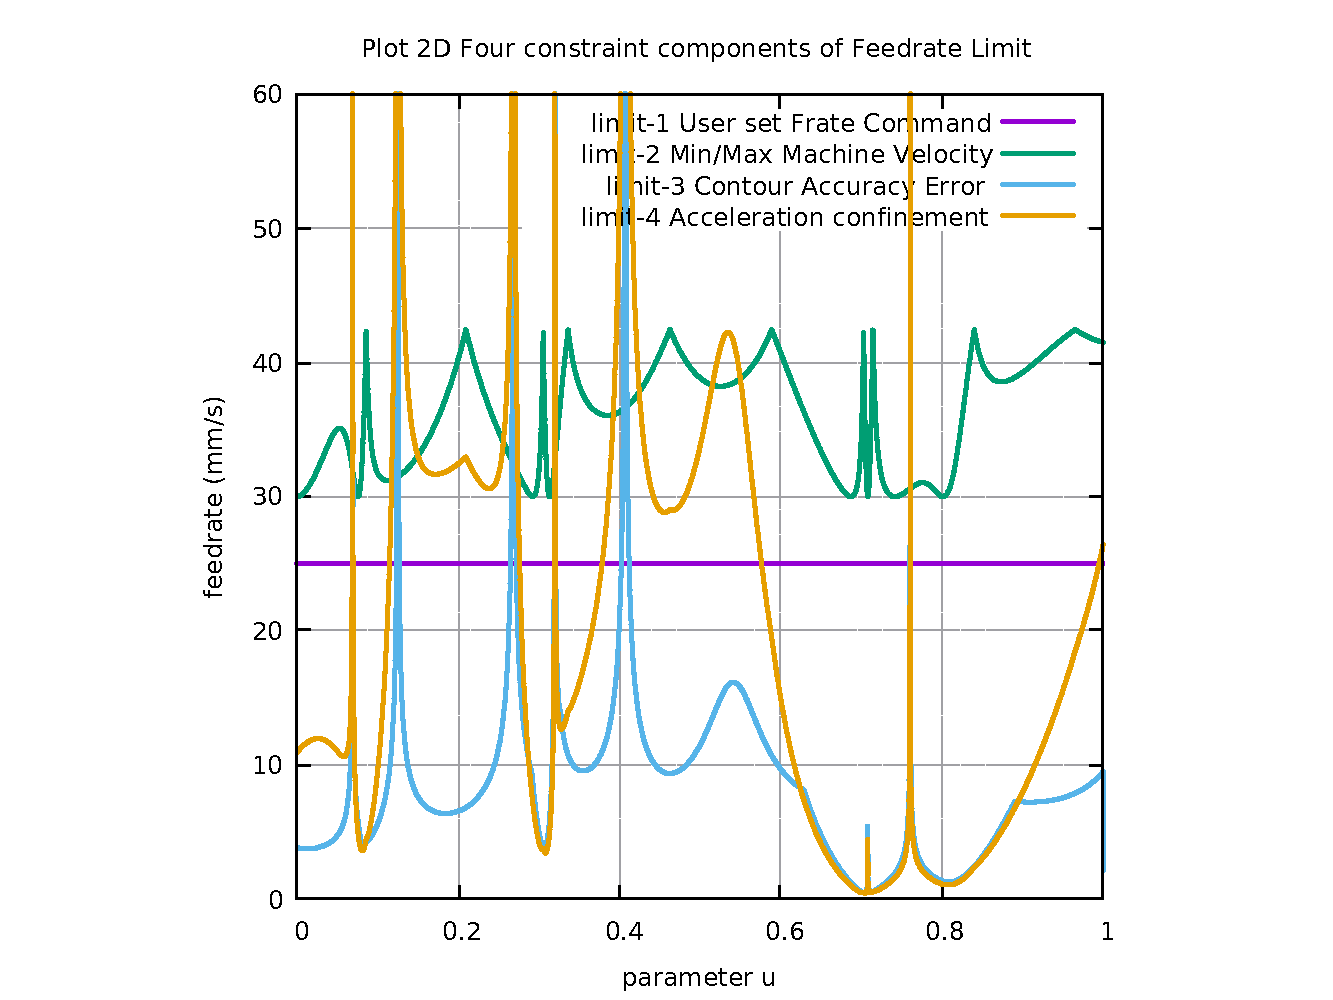
\includegraphics[width=1.00\textwidth]{Chap4/appendix/app-SnaHyp/plots/33-img-SnaHyp-FC30-Four-Components-FeedrateLimit.pdf}
\end{figure}


\begin{figure}
	\caption     {SnaHyp FC28 Four Components FeedrateLimit}
	\label{34-img-SnaHyp-FC28-Four-Components-FeedrateLimit.pdf}
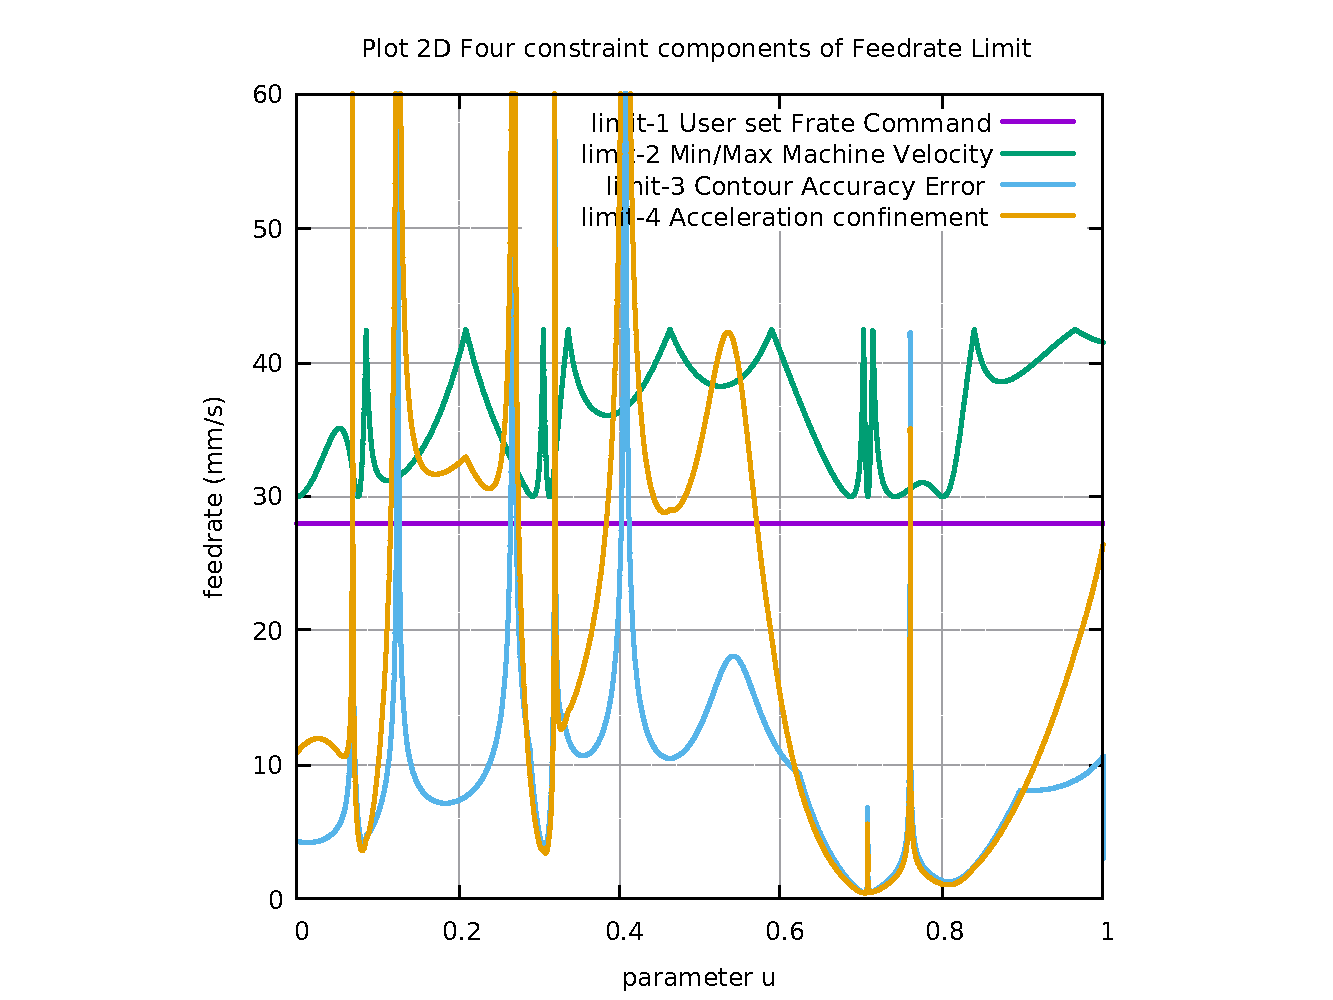
\includegraphics[width=1.00\textwidth]{Chap4/appendix/app-SnaHyp/plots/34-img-SnaHyp-FC40-Four-Components-FeedrateLimit.pdf}
\end{figure}


%% =======================================
\clearpage
\pagebreak

\begin{figure}
	\centering
	\caption     {SnaHyp Histogram Points FC10 FC20 FC30 FC40}
	\label{35-img-SnaHyp-Histogram-Points-FC10-FC20-FC30-FC40.pdf}
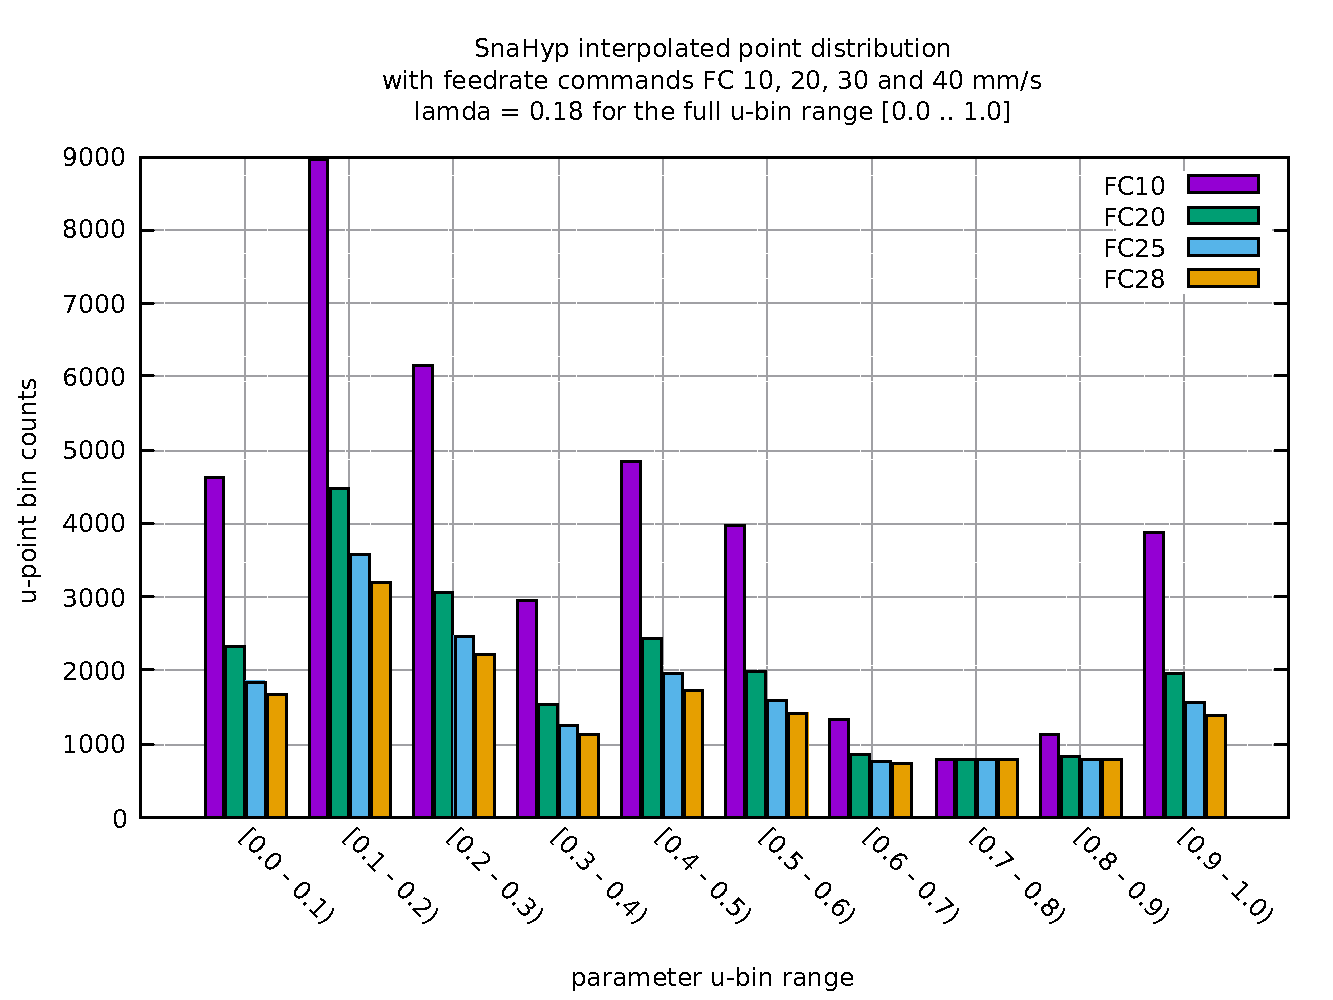
\includegraphics[width=1.00\textwidth]{Chap4/appendix/app-SnaHyp/plots/35-img-SnaHyp-Histogram-Points-FC10-FC20-FC30-FC40.pdf} 
\end{figure}


\begin{table}[ht]
%% \begin{center}
\caption    {SnaHyp Table distribution of interpolated points}
\label  {tab-SnaHyp Table distribution of interpolated points}
	
%% IMPORTANT TO SCALEBOX BELOW
\scalebox{0.80}{
		
%% START COPY AND PASTE BELOW HERE
%% FROM \begin{tabular} UNTIL \end{tabular)
%% Note: adjust last p{} to get line width correct
		
\begin{tabular}{ p{4.5cm} p{1.5cm} p{1.5cm} p{1.5cm} p{7.50cm} }
\hline
	&		&		&		&		\\
BINS	&	FC10	&	FC20	&	FC25	&	FC28	\\
&		&		&		&		\\
0.0 - 0.1	&	4631	&	2317	&	1856	&	1666	\\
0.1 - 0.2	&	8961	&	4480	&	3584	&	3200	\\
0.2 - 0.3	&	6140	&	3074	&	2470	&	2213	\\
0.3 - 0.4	&	2960	&	1526	&	1257	&	1146	\\
0.4 - 0.5	&	4860	&	2431	&	1945	&	1736	\\
0.5 - 0.6	&	3973	&	1987	&	1589	&	1420	\\
0.6 - 0.7	&	1324	&	841	&	769	&	744	\\
0.7 - 0.8	&	794	&	794	&	794	&	796	\\
0.8 - 0.9	&	1141	&	828	&	798	&	791	\\
0.9 - 1.0	&	3888	&	1945	&	1556	&	1390	\\
&		&		&		&		\\
Tot Counts	&	38672	&	20223	&	16618	&	15102	\\
&		&		&		&		\\
\hline	
\end{tabular}
		
%% END COPY AND PASTE ABOVE HERE
		
}   %% IMPORTANT FOR SCALEBOX CLOSING
	
\end{table}
%% \end{landscape}

%% SnaHyp SUMMARY TABLE
%% ========================================================
\clearpage
\pagebreak
\begin{landscape}
	
\begin{table}[ht]
%% \begin{center}
\caption       {SnaHyp Table FC10-20-30-40 Run Performance data}
\label{tab-app4-SnaHyp-Table-FC10-20-30-40-Run-Performance-data}
		
%% IMPORTANT TO SCALEBOX BELOW
\scalebox{0.90}{
			
%% START COPY AND PASTE BELOW HERE
%% FROM \begin{tabular} UNTIL \end{tabular)
			
\begin{tabular}{ p{0.2cm} p{8.80cm} p{4.00cm} p{4.0cm} p{4.00cm} p{4.0cm}}
	\hline
	&		&		&		&		&		\\
	1	&	Curve Type	&	SNAHYP	&	SNAHYP	&	SNAHYP	&	SNAHYP	\\
	2	&	User Feedrate Command FC(mm/s)                   	&	FC10	&	FC20	&	FC25*	&	FC28**	\\
	3	&	User Lamda Acceleration Safety Factor	&	0.18	&	0.18	&	0.18	&	0.18	\\
	&		&		&		&		&		\\
	4	&	Total Iterpolated Points (TIP)	&	38672	&	20223	&	16618	&	15102	\\
	5	&	Total Sum-Chord-Error (SCE) (mm)	&	2.846873175820E-03	&	4.002975369043E-03	&	4.459254922025E-03	&	4.700022719935E-03	\\
	6	&	Ratio 1 = (SCE/TIP) = Chord-Error/Point	&	7.361778014067E-08	&	1.979515067275E-07	&	2.683549932012E-07	&	3.112391709116E-07	\\
	&		&		&		&		&		\\
	7	&	Total Sum-Arc-Length (SAL) (mm)	&	3.779474877648E+02	&	3.779592539969E+02	&	3.779667959094E+02	&	3.779678653378E+02	\\
	8	&	Total Sum-Chord-Length (SCL) (mm)	&	4.789870865777E+02	&	4.789986994127E+02	&	4.790063715425E+02	&	4.790071286890E+02	\\
	9	&	Difference = (SAL – SCL) (mm)	&	-1.010395988129E+02	&	-1.010394454158E+02	&	-1.010395756332E+02	&	-1.010392633512E+02	\\
	10	&	Percentage Difference = (SAL – SCL)/SAL	&	-2.673376648446E+01	&	-2.673289365118E+01	&	-2.673239467770E+01	&	-2.673223641934E+01	\\
	&		&		&		&		&		\\
	11	&	Ratio 2 = (SCE/SCL) = Chord Error/Chord-Length	&	5.943528031539E-06	&	8.356965006276E-06	&	9.309385400583E-06	&	9.812009964860E-06	\\
	&		&		&		&		&		\\
	12	&	Total Sum-Arc-Theta (SAT) (rad)	&	5.483921922253E+02	&	5.514331568816E+02	&	5.514225232921E+02	&	5.481728747328E+02	\\
	13	&	Total Sum-Arc-Area (SAA) (mm2)	&	2.706870610425E-01	&	2.760007501922E-01	&	2.777614243305E-01	&	2.754368695310E-01	\\
	&		&		&		&		&		\\
	14	&	Ratio 3 = (SAA/SCL) = Arc-Area/Chord-Length	&	5.943528031539E-06	&	8.356965006276E-06	&	9.309385400583E-06	&	9.812009964860E-06	\\
	&		&		&		&		&		\\
	15	&	Average-Chord-Error (ACE) (mm)	&	7.361778014067E-08	&	1.979515067275E-07	&	2.683549932012E-07	&	3.112391709116E-07	\\
	16	&	Average-Arc-Length (AAL) (mm)	&	9.773408698114E-03	&	1.869049817016E-02	&	2.274579020939E-02	&	2.502932688814E-02	\\
	17	&	Average-Chord-Length (ACL) (mm)	&	1.238620895704E-02	&	2.368700916886E-02	&	2.882628462072E-02	&	3.172022572604E-02	\\
	18	&	Average-Arc-Theta (AAT) (rad)	&	1.418096744913E-02	&	2.726897225208E-02	&	3.318424043402E-02	&	3.630043538393E-02	\\
	19	&	Average-Arc-Area (AAA) (mm2)	&	6.999742986798E-06	&	1.364853872971E-05	&	1.671549764280E-05	&	1.823964436336E-05	\\
	&		&		&		&		&		\\
	20	&	Algorithm actual runtime on computer (ART) (s) 	&	18.694644926	&	16.525007035	&	16.49022576	&	16.65385009	\\
	&		&		&		&		&		\\
\hline	
\end{tabular}

			
%% END COPY AND PASTE		
}   %% IMPORTANT FOR SCALEBOX CLOSING
		
\end{table}
\end{landscape}

%% =======================================
\clearpage
\pagebreak
